\documentclass[12pt]{article}
\usepackage[utf8]{inputenc}
\usepackage{adjustbox}
\usepackage{algorithm}
\usepackage{algpseudocode}
\usepackage{amsmath}
\usepackage[titletoc]{appendix}
\usepackage{array}
\usepackage{bbm}
\usepackage{color}
\usepackage{comment}
\usepackage{float}
\usepackage{gensymb}
\usepackage[top=1in, bottom=1in, left=1.25in, right=1.25in]{geometry}
\usepackage{graphicx}
\usepackage{listings}
\usepackage{mathtools}
\usepackage{multicol}
\usepackage{needspace}
\usepackage{placeins}
\usepackage{subcaption}
\usepackage{tablefootnote}
\usepackage{textcomp}
\usepackage{tikz}
\usepackage{titlesec}
\usepackage{titling}
\usepackage{url}

\usetikzlibrary{matrix,shapes,arrows,positioning,chains}
\tikzset{
decision/.style={
    diamond,
    draw,
    text width=4em,
    text badly centered,
    inner sep=0pt
},
block/.style={
    rectangle,
    draw,
    text width=10em,
    text centered,
    rounded corners
},
cloud/.style={
    draw,
    ellipse,
    minimum height=2em
},
descr/.style={
    fill=white,
    inner sep=2.5pt
},
connector/.style={
    -latex,
    font=\scriptsize
},
rectangle connector/.style={
    connector,
    to path={(\tikztostart) -- ++(#1,0pt) \tikztonodes |- (\tikztotarget) },
    pos=0.5
},
rectangle connector/.default=-2cm,
straight connector/.style={
    connector,
    to path=--(\tikztotarget) \tikztonodes
}
}


\title{\large{Empirical assessment of adaptation to chronic illness} \\{Can time heal all wounds?}}

\author{Anne de Hond }
\date{August 2017}

\begin{document}
\begin{titlingpage}
    \begin{center}
        \vspace*{1cm}
        
        \textbf{\huge Empirical assessment of adaptation to chronic illness}\\
        \vspace{0.5cm}
        \textbf{\Large Can time heal all wounds?}\\
        \vspace{2cm}
        \Large{Anne de Hond   \\
        428033}      
     \end{center}   
        
                
        \vspace{10cm}
        
        {\normalsize \noindent Erasmus University Rotterdam}\\
        {\textit{\small MSc Econometrics and Management Science\\
        \indent specialisation Econometrics}}\\
        {\small Master's Thesis Econometrics \quad\quad\quad\quad\quad\quad\quad\quad\quad\quad\quad\quad\quad\quad\quad\quad\quad\quad\quad\quad\quad\quad\quad \textbf{\textcolor{red}{date}}}\\


\end{titlingpage}

        \begin{abstract}
        \noindent Introduction \\
        In health state evaluations, members of the general public are inclined to estimate a larger negative impact of a health impairment compared to patients themselves. This adds to the controversy about the type of health state preferences that should be used. The difference in the patient's experience and the public's ideation is often attributed to adaptation. This master thesis studies adaptation to chronic disability in a large longitudinal data set.\\
        \\
        \noindent Method \\
        I select over 5000 respondents of the Survey of Health, Ageing and Retirement in Europe (SHARE) who develop a chronic illness and disabilities during the span of the 5 waves of data collection. Adaptation is analyzed for outcome variables self-perceived health and life satisfaction. Self-perceived health is measured on a 5 point Likert scale, with anchors poor to excellent health and life satisfaction on a numbered scale ranging 1 to 11, with anchors very dissatisfied, very satisfied. In order to examine the effect of time since the onset of disability on self-perceived health and life satisfaction, a fixed effects ordered probit model and a fixed effects linear model are recommended in the literature. I use a fixed effects ordered logit model as the dependent variable is measured on an ordinal scale and the probit model is prone to misspecification. For comparison reasons, I also analyze the fixed effects probit and linear model.\\
        \\
        Results \\
        Over 13000 observations for life satisfaction and over 15000 for self-perceived health are used. Self-perceived health significantly decreases when the disabilities occur, but life satisfaction remains the same. Supportive evidence for adaptation in the life satisfaction analysis was found, but not in that for self-perceived health. \\
        \\
        Discussion\\
        It is possible that the effect of adaptation to chronic disability in self-perceived health can only be found after a longer duration than that measured here. The difference might also be explained by the contextualization of the response variables, where the question on self-perceived health is more focused on health limitations and the question on life satisfaction on general well-being. 
     \end{abstract}
\newpage
\tableofcontents
\newpage

%%%%%%%%%%%%%%%%%%%%%%%%%%%%%%%%%%%%%%%%%%%%%%%%%%%%%%%%%%%%%%%%%%%%%%%%%%%%%%%%%%%%%%%%%%%%%%%%%%%%%%%%%%%%%%%%%%%%%%%%%%%%%%%%%%%%%%%%%%%%%%%%

\section{Introduction}

Health state evaluations \textcolor{red}{adaptatie belangrijk voor onder andere health economics evaluations en epidemiologisch onderzoek, theoretisch kader adaptatie, geen secundaire literatuur quoten} have become increasingly important to policy makers concerned with the allocation of health care resources (Menzel, Dolan, Richardson \& Olsen, 2002; Versteegh \& Brouwer, 2016). These economic evaluations are requested in many countries to inform pricing, reimbursing and funding decisions (Cub\'i-Moll\`a, Jofre-Bonet \& Serra-Sastre, 2016). The evaluations are usually based on respondents' preferences for being in an impaired health state compared to being completely healthy. Interestingly, health state preferences of the general public (consisting of generally healthy individuals) do not necessarily coincide with those of patients. Members of the general public are inclined to estimate a larger negative impact of health impairments compared to the health state appraisals of the patients themselves (Sackett \& Torrance, 1978; Krahn et al., 2003; Peeters \& Stiggelbout, 2010). Thus, the discussion dedicated to the question which group of people should be consulted to obtain these measurements is not trivial. %Boyd, Sutherland, Heasman, Trichler \& Cummings, 1990; Hurst et al., 1994; ; Zethraeus and Johannesson, 1999

In the Netherlands, health state evaluations of the general public are preferred (Zorginstituut Nederland, 2016), even though patient health state evaluations are more informative about the subjective impact of a certain health state. The general concern with patient health state evaluations is that they are potentially biased due to ``response shifts". The idea being that the meaning of a patient's self-evaluation has changed due to a change in internal standards, values, or conceptualization of quality of life, leading to a shift in the patient's reference point (Sprangers \& Schwartz, 1999). In contrast, members of the general public reason from the same reference point of being in full health and are thought to have a uniform representation of the `distance' between their own healthy state and the health impairment. Thus, an argument in favour of health state preferences of the general public is that they lend themselves to universally applicable valuations.

%However, the discrepancy in patient and general public preferences for health states is likely driven by the fact that the general public fails to take the other factors into account that may affect subjective health. In this sense, they are `wrong' when predicting their own preferences compared to the actual patients' reports, which can be used as an argument for choosing patient preferences. 
Adaptation to impaired health states is a particular realization of response shift (Cub\'i-Moll\`a, Jofre-Bonet \& Serra-Sastre, 2016). The difference in the patient's experience and the public's ideation of certain health states is often attributed to adaptation. Frederick and Loewenstein describe adaptation as ``a reduction in the affective intensity of favorable and unfavorable circumstances" (1999, p.302). A proper understanding of the dynamics governing the health state preferences of patients could be highly beneficial to the discussion on health state measurements. In particular, the empirical assessment of the adaptation process could help explain the difference between patient and public health state measurements and create insight into the changes of patients' self-perceived health over the course of the disability. 

Adaptation to health states has been widely studied by psychologists and experimental economists. However, there only appears to be a small (yet growing) set of high-quality studies that have empirically examined adaptation. Early studies investigating adaptation to impaired health states predominantly employ cross-sectional methods. Note that this means no conclusions can be drawn regarding the effect of time since diagnosis on subjective health and hence these results cannot be used as evidence for adaptation within patients. However, the cross-sectional analyses enable a comparison of health state measurements across different groups of people. The counter-intuitive results show that patients with serious health limitations report well-being or self-reported health levels that are notably above the health state appraisals of healthy subjects as was previously mentioned (Sackett \& Torrance, 1978; Krahn et al., 2003; Peeters \& Stiggelbout, 2010). Moreover, certain studies even found that patient well-being is only marginally lower than that of healthy subjects (Brickman, Coates \& Janoff-Bullman, 1978; Schulz \& Decker, 1985; Tyc, 1992).

Recent studies have used panel data in order to examine adaptation to chronic infirmity from the moment of diagnosis. Their empirical evidence does not provide unambiguous support for the occurrence or level of adaptation. Lucas (2007) does not find any adaptation in two large panel data sets. In his study, multilevel models were used to measure adaptation in long-term disabled subjects on life satisfaction. On the other hand, Oswald and Powdthavee (2008) cannot replicate Lucas' findings \textcolor{red}{leg uit waarom Oswald en Lucas verder niet beschreven worden} using a fixed effects model for self-reported life satisfaction, whilst analyzing the same data sets. They find a considerable level of adaptation and suggest that the differing results are due to a difference in the respective methodologies, with the multilevel model used by Lucas being technically closer to a random effects model. Finally, Cub\'i-Moll\`a, Jofre-Bonet and Serra-Sastre (2016) do find some evidence for adaptation to self assessed health. They make use of a dynamic fixed effects probit model by utilizing Wooldrigde's (2005) approach. The authors only find a significant effect of duration since the onset of a long-standing illness after 20 years.  

It is the objective of this thesis to study adaptation to chronic health limitations. I hypothesize that time since the onset of the chronic disability is positively related to the probability of reporting better health and life satisfaction. To this aim, the effect of adaptation, assessed through the time an individual has experienced limitations with instrumental activities of daily living (IADL) and the severity of these limitations, is analyzed for both self-perceived health and life satisfaction. I hope to establish changes in either of these constructs that can be attributed to the adaptation response shift process as a function of time spend with a chronic disability. The main assumption is that changes in either self-perceived health or life satisfaction can indeed be attributed to the adaptation mechanism, whatever the nature of the contributing factors. The intensity of the underlying impaired health condition is controlled for by the number of limitations with (IADL), which is indicative of the severity of the chronic disability. In doing so, the health state of the respondents is allowed to fluctuate over time. Furthermore, I control for potential other shocks to subjective health and life satisfaction by adding socioeconomic covariates like marital status and labour-force status.   

The data used for this analysis is obtained from the SHARE (Survey of Health, Ageing and Retirement in Europe) database. It is a panel data set consisting of individuals aged 50 and over spanning 6 waves. I find that a longer duration is related to a higher probability of being satisfied with life, but not with the probability of reporting a better self-perceived health. 

This thesis contributes to the existing literature in that it uses panel data as opposed to a cross-sectional model. In doing so, the trajectory of adaptation over time can be studied and I can control for individual heterogeneity. I employ a fixed effects ordered logit model, which has to my knowledge not been used for studying adaptation. This nonlinear model exploits the ordering of the dependent variable whilst allowing it to be discrete. It consistently estimates the parameters. Furthermore, the duration of the chronic disability is measured by dummy variables, permitting the effect of adaptation since the onset of the chronic limitations to be nonlinear. In addition, adaptation is analyzed for both self-perceived health and life satisfaction, since the effect could differ per outcome measure and no research has looked into this potential difference. Finally, the analysis is not limited to individuals whose latent health is assumed to stay constant. By broadening my selection to those reporting differing levels in the number of limitations with IADL, I can apply the results to a wider scope of health conditions, like diseases that deteriorate over time. In sum, this thesis aims to add new insights to the investigation of adaptation to chronic disability. The results can be used to inform members of the general public about the changes in the health perception of patients, so that they can incorporate this into their health state preferences. 

This thesis consists of the following sections. The next section contains the methodology focusing on three econometric models of interest. Section 3 presents the data set and results, including an investigation regarding the robustness of the results. The final section provides a conclusion and a discussion on the limitations with suggestions for future research.  

\textcolor{red}{advantages of using IADL}

%Moreover, I will use the number of limitations with instrumental activities of daily living (IADL) as the measure of incidence and intensity of disability or illness. I believe that this is the appropriate choice for this particular study, since I am interested in adaptation to health problems in general and limitations with IADL always imply general health problems. 
%\textcolor{red}{something about argument in favour of patient preferences} However, not all of the underlying mechanisms driving adaptation are laudable. Menzel, Dolan, Richardson and Olsen (2002) identify eight elements of adaptation. `Skill enhancement', `activity adjustment', 'substantive goal adjustment' and `altering conceptions of health' can be seen as laudable achievements and can be used to argue in favour of adaptation shaped preferences. On the other hand, `cognitive denial', `suppressed recognition of full health' and `lowered expectations' are denoted as negative elements and, as Versteegh and Brouwer (2016) also point out, they are perception biases rather than adjustments of oneself. Finally, `heightened stoicism' is not particularly admirable nor regrettable. Hence, the nature of the mechanisms thought to be predominant ought to guide the importance attached to patient based preferences. Nonetheless, patient preferences should not be disregarded on the basis of adaptation alone.  

%To quote Frederick and Loewenstein: ``the hedonic deterioration that is commonly observed does not provide evidence that adaptive processes are not occurring - only that they are not occurring fast enough to keep pace with the progression of the disease" (1999, p. 312).
\FloatBarrier

%%%%%%%%%%%%%%%%%%%%%%%%%%%%%%%%%%%%%%%%%%%%%%%%%%%%%%%%%%%%%%%%%%%%%%%%%%%%%%%%%%%%%%%%%%%%%%%%%%%%%%%%%%%%%%%%%%%%%%%%%%%%%%%%%%%%%%%%%%%%%%%%

\section{Literature review}


%%%%%%%%%%%%%%%%%%%%%%%%%%%%%%%%%%%%%%%%%%%%%%%%%%%%%%%%%%%%%%%%%%%%%%%%%%%%%%%%%%%%%%%%%%%%%%%%%%%%%%%%%%%%%%%%%%%%%%%%%%%%%%%%%%%%%%%%%%%%%%%%

\section{Methods}

A perusal of the adaptation literature brings to light the myriad of choices involved in the econometric modelling of the adaptation process. In order to explain my preference for the fixed effects ordered logit specification, I will first generally compare and contrast two methods employed in the literature with my proposed model. The two particular empirical strategies under consideration here are presented in Clark, D'Ambrosio and Ghislandi (2016) and Cub\'i-Moll\`a, Jofre-Boner and Serra-Sastre (2016). 

A schematic overview of the most important features of the logit model and the two models from the literature can be found in table \ref{modelchoice}. First of all, note that all model specifications here assume fixed effects, meaning that the individual heterogeneous terms might be correlated with the regressors. Secondly, both the ordered logit model proposed in this thesis and the ordered probit model presented by Cub\'i-Moll\`a, Jofre-Boner and Serra-Sastre are nonlinear. These nonlinear model specifications are attractive, since they account for the discrete nature of the outcome variable (subjective health or life satisfaction), whilst still incorporating its ordered structure. However, in the estimation of these model coefficients, the unobserved heterogeneity cannot simply be removed by performing a linear transformation, like the within transformation that can be applied to the OLS fixed effects model proposed by Clark, D'Ambrosio and Ghislandi. As a consequence, the fixed effects cannot be estimated consistently under a fixed number of time periods. Even as the number of individuals grows without bound, the number of parameters to be estimated also goes to infinity. This is referred to as the incidental parameters problem (Neyman \& Scott, 1948). In short panels (a small number of observed time periods), this can lead to severe bias in the estimation of the regression parameters (Green, 2004). The ordered logit and ordered probit approaches discussed here both have distinct ways of handling this problem.

The ordered probit model put forward by Cub\'i-Moll\`a, Jofre-Boner and Serra-Sastre has, in addition to fixed effects, a dynamic structure. In order to deal with both the incidental parameters problem and the initial conditions problem created by the dynamics, they make use of a parameterization of the fixed effects as a function of the regressors following Wooldridge (2005). Even though their solution is parsimonious and easy to implement, the parameterization is prone to misspecification. Hence, I propose a technique based on the principles of the conditional logit estimator. The estimator in question is described in Baetschmann, Staub, and Winkelmann (2015). It effectively eliminates the fixed effects in an ordered logit model and yields consistent estimates, without having to parameterize the fixed effects.  

Finally, the analyses by Clark, D'Ambrosio and Ghislandi and Cub\'i-Moll\`a, Jofre-Boner and Serra-Sastre assume a different functional form for the adaptation process. Both methodologies measure adaptation by means of the duration since the onset of the life event, but only Clark, D'Ambrosio and Ghislandi allow the effect to be nonlinear by constructing dummy variables. These dummy variables correspond to consecutive time segments indicative of how long ago somebody experienced the negative life event. I also believe that the continuous functional form for adaptation of Cub\'i-Moll\`a, Jofre-Boner and Serra-Sastre is too restrictive and use the dummy specification outlined here. 

\begin{table}[htbp]
\centering
\footnotesize
\caption{Econometric strategies for modelling adaptation}
\label{modelchoice}
\begin{tabular}{l lll}
\hline
& \multicolumn{1}{c}{De Hond (2017)} & \multicolumn{1}{c}{Clark, D'Ambrosio} & \multicolumn{1}{c}{Cub\'i-Moll\`a, Jofre-Boner} \\
& \multicolumn{1}{c}{} & \multicolumn{1}{c}{\& Ghislandi (2016)} & \multicolumn{1}{c}{\& Serra-Sastre (2016)}\\\hline\hline
Model specification                & FE ordered logit            & FE OLS               & FE ordered probit \\
Functional form adaptation         & Dummy variables             & Dummy variables      & Continuous      \\
Parameterization of FE             & No                          & No                   & Yes   \\
\hline
\end{tabular}
\caption*{\footnotesize{\textit{Note.} FE stands for fixed effects.}}
\end{table}

In sum, the main features of my proposed fixed effects ordered logit specification can be found in the first column of table \ref{modelchoice}. Next, an in depth discussion devoted to the econometric theory of this ordered logit model is provided.

\FloatBarrier

%%%%%%%%%%%%%%%%%%%%%%%%%%%%%%%%%%%%%%%%%%%%%%%%%%%%%%%%%%%%%%%%%%%%%%%%%%%%%%%%%%%%%%%%%%%%%%%%%%%%%%%%%%%%%%%%%%%%%%%%%%%%%%%%%%%%%%%%%%%%%%%%

\subsection{Fixed effects ordered logit model}
The fixed effects ordered logit estimation utilized here is based on the ``blow-up and cluster" (BUC) estimator proposed by Baetschmann, Staub and Winkelmann (2015). The ordered logit specificaiton assumes the existence of a latent response variable according to:

\begin{equation}
    Y_{it}^* = C_{it}'\theta + D_{it}'\delta + IADL_{it}\gamma + \alpha_{i} + \varepsilon_{it}, \quad i=1,\ldots,N, \quad t=1,\ldots,T.
\end{equation}

Here, $Y_{it}^*$ is the respondent's latent self-perceived health or life satisfaction. The variables of interest are the number of limitations with instrumental activities of daily living (IADL), $IADL_{it}$, and duration, $D_{it}$, measured by dummies indicating the time since the onset of the limitations. I expect a negative effect for $IADL_{it}$, but a positive effect for at least one of the dummies contained by $D_{it}$. $C_{it}$ consists of a number of sociodemographic covariates. For the remainder of this discussion, I shorten the notation by grouping the regressors in the vector $X_{it} = (C'_{it},D'_{it},IADL_{it})'$ and the parameters by $\beta = (\theta',\delta',\gamma)'$. Lastly, $\alpha_{i}$ is the individual specific fixed effect and I assume that the error term follows a logistic distribution:

\begin{equation}
    F(\varepsilon_{it}|X_{it},\alpha_{i}) = \frac{exp(\varepsilon_{it})}{1+exp(\varepsilon_{it})} \equiv \Lambda(\varepsilon_{it})
\end{equation}

The observed self-perceived health or life satisfaction, denoted by $Y_{it}$, is constructed from $Y_{it}^*$ as follows:

\begin{equation}
    Y_{it} = k \quad \textrm{if } \tau_{ik-1}<Y_{it}^*\leq\tau_{ik}, \quad k=1,\ldots,K.
\end{equation}

\noindent The thresholds between categories $k-1$ and $k$ can be individual specific, with $\tau_{i0}=-\infty$ and $\tau_{iK}=\infty$. 

The probability for individual $i$ at time $t$ of reporting outcome $k$ is given by 

\begin{equation}
    P(Y_{it}=k|X_{it},\alpha_{i}) = \Lambda(\tau_{ik}-X_{it}'\beta-\alpha_{i}) - \Lambda(\tau_{ik-1}-X_{it}'\beta-\alpha_{i}).
    \label{logitprob}
\end{equation}


\begin{equation}
    P_{i}^k(\beta) = P(d_{i}^k=j_{i}|\sum_{t=1}^{T}{d_{it}^k=g_{i}}) = \frac{exp(j_{i}'X_{i}\beta)}{\sum_{j\in B_{i}}{exp(j'X_{i}\beta)}}.
    \label{logitprob2}
\end{equation}

Here, the sum of all the outcomes over time, $\sum_{t=1}^{T}{d_{it}^k}=g_{i}=\sum_{t=1}^{T}{j_{it}}$, is a sufficient statistic for $\alpha_{i}$, since the probability in equation \ref{logitprob2} is independent of $\alpha_{i}$ and the thresholds. Moreover, $X_{i}$ is a $T\times M$ matrix, with $M$ the number of regressors and row $t$ equal to $X_{it}$. The sum in the denominator of equation \ref{logitprob2} concerns the set $B_{i}$ which consists of all vectors $j$ of length $T$ that have as many elements equal to one as the observed vector $j_{i}$ of individual $i$: 

\[
    B_{i} = \Bigg\{ j \in \{0,1\}^T | \sum_{t=1}^{T}{j_{t}}=g_{i} \Bigg\}.
\]

The resulting conditional log likelihood is given by 
\begin{equation}
    LL^k(b) = \sum_{i = 1}^{N} log(P_{i}^k(b)).
    \label{LL}
\end{equation}

\noindent The maximization of this likelihood function for a dichotomized dependent variable at any cut-off point $k$ has been shown to be consistent by Chamberlain (1980) and will therefore be referred to as the Chamberlain estimator denoted by $\hat{\beta}^k$. The first order derivatives and individual Hessians used for this optimization can be found in appendix A.1. 

Note that individuals with constant $d_{it}^k$ do not contribute to the conditional log likelihood, since $P(d_{it}^k=1|\sum_{t=1}^{T}{d_{it}^k}=T) = P(d_{it}^k=0|\sum_{t=1}^{T}{d_{it}^k}=0)=1$. Hence, it is worthwhile to obtain $\beta$ estimates acquired with Chamberlain estimators using different cut-off points $k$, since the group of individuals contributing to the likelihood function is likely to change for different cut-off points. In fact, if we employ all possible $K-1$ Chamberlain estimators of $\beta$, each individual will contribute at least once to a likelihood function, as long as the observed $Y_{it}$'s of the individual in question are not constant.

The BUC estimator proposed by Baetschmann, Staub and Winkelmann (2015) is based on the maximization of the sum of all possible $K-1$ Chamberlain likelihood functions:

\begin{equation}
    LL^{BUC}(b) = \sum_{k=2}^{K}{LL^k(b)}, 
    \label{LL2}
\end{equation}

where $LL^k(b)$ is defined in equation \ref{LL}. By exploiting the information provided by the different configurations of individuals for different cut-off points, the BUC estimator is more efficient than the Chamberlain estimator. The BUC estimator, $\hat{\beta}^{BUC}$, maximizes the likelihood in equation \ref{LL2} under the restriction that $\hat{\beta}^2=\ldots=\hat{\beta}^K$. Since the individual Chamberlain estimators are consistent, it is easy to verify the consistency of the BUC estimator. The first order derivatives of the Chamberlain estimators converge to 0 at the true parameter, which means that the sum of the derivatives - equalling the first order derivative of the BUC log likelihood - will converge to 0 as well at its optimum. Given the concavity of the objective function, this ensures that $\hat{\beta}^{BUC}$ converges to $\beta$.

We need to cluster the standard errors at the individual level, due to the constructed dependency between the observations. Hence, the information matrix equality used for the regular maximum likelihood approach is not valid and a cluster robust variance estimator should be used based on the following asymptotic variance (the limiting variance of $\sqrt{n}(\hat{\beta}^{BUC}-\beta)$):

\begin{equation}
    Avar(\hat{\beta}^{BUC}) = \Bigg\{ \sum_{k=2}^{K}{E(H_{i}^{k}(\beta))} \Bigg\}^{-1} \Bigg[ \sum_{k=2}^{K}\sum_{l=2}^{K}{E(s_{i}^k(\beta)s_{i}^l(\beta)')} \Bigg] \Bigg\{ \sum_{k=2}^{K}{E(H_{i}^{k}(\beta))} \Bigg\}^{-1}.
\end{equation}

\noindent Here, $H_{i}^k(\beta)$ denote the individual Hessians and $s_{i}^k(\beta)$ the first order derivatives with respect to the Chamberlain likelihood function in equation \ref{LL}. In the analysis, the expectations are replaced by their sample analogs and the parameters by their estimated values.

Finally, from the $\beta$ estimates we can derive the statistical significance of the effect of the regressors on the probability of reporting better self-perceived health or life satisfaction. They cannot, however, be interpreted in terms of the size of this effect. For this type of interpretation the marginal effects are required. In the subsequent analysis, I use the marginal effect on $P(Y_{it}>k) = 1 - \Lambda(\tau_{ik}-X_{it}'\beta-\alpha_{i})$, since the sign of the regression estimate then always concurs with that of the corresponding marginal effects. The general formula for the marginal effect of the $l$th regressor on the probability that a respondent reports an outcome higher than category $k$ is: 

\begin{equation}
    \frac{\partial P(Y_{it}>k|X_{it},\alpha_{i})}{\partial X_{it}} = \Lambda_{ik}(1-\Lambda_{ik})\beta_{l},
\end{equation}

with $\Lambda_{ik} = \Lambda(\tau_{ik} - X_{it}'\beta - \alpha_{i})$. Usually, the average of the effects is calculated to aid the interpretation. Unfortunately, average marginal effects for $P(Y_{it}>k)$ cannot be calculated directly, since $\tau_{ik}$ and $\alpha_{i}$ are not estimated by the BUC estimator. However, I will approximate the required probabilities with the sample probabilities:

These are computed by summing the number of observations in the categories larger than $k$ and dividing this by the total number of observations. Even though the resulting marginal effects are approximations, I expect them to aid the general interpretation of the results. 

%%%%%%%%%%%%%%%%%%%%%%%%%%%%%%%%%%%%%%%%%%%%%%%%%%%%%%%%%%%%%%%%%%%%%%%%%%%%%%%%%%%%%%%%%%%%%%%%%%%%%%%%%%%%%%%%%%%%%%%%%%%%%%%%%%%%%%%%%%%%%%%%

\subsection{The OLS and probit models}

In addition to the fixed effects ordered logit model, I have also analyzed adaptation to chronic disability by following the proposed model specifications of Clark, D'Ambrosio and Ghislandi (2016) and Cub\'i-Moll\`a, Jofre-Boner and Serra-Sastre (2016). In light of the previous comparison of these three models, I will examine whether the discussed differences in modelling strategies affect the results. Next, the econometric foundation of these two supplementary models is outlined shortly. 

%%%%%%%%%%%%%%%%%%%%%%%%%%%%%%%%%%%%%%%%%%%%%%%%%%%%%%%%%%%%%%%%%%%%%%%%%%%%%%%%%%%%%%%%%%%%%%%%%%%%%%%%%%%%%%%%%%%%%%%%%%%%%%%%%%%%%%%%%%%%%%%%

\subsubsection{Fixed effects OLS model}

The fixed effects OLS model is featured in the study by Clark, D'Ambrosio and Ghislandi (2016) who use it to investigate adaptation to poverty. The regression equation is:
\begin{equation}
\label{FE}
    Y_{it} = C_{it}'\theta + D_{it}'\delta + IADL_{it}'\gamma + \alpha_{i} + \varepsilon_{it},
\end{equation}
with $Y_{it}$ the self-reported health or life satisfaction, $C_{it}$ a vector with covariates, $D_{it}$ a vector with dummy variables capturing the time since onset of the chronic disability and $IADL_{it}$ the number of limitations with IADL. The coefficients can be estimated by means of ordinary least squares linear fixed effects. Additional statistics can be derived with the standard fixed effects calculations. 

%%%%%%%%%%%%%%%%%%%%%%%%%%%%%%%%%%%%%%%%%%%%%%%%%%%%%%%%%%%%%%%%%%%%%%%%%%%%%%%%%%%%%%%%%%%%%%%%%%%%%%%%%%%%%%%%%%%%%%%%%%%%%%%%%%%%%%%%%%%%%%%%

\subsubsection{Fixed effects ordered probit model}

The second model is based on the ordered fixed effects probit model put forward by Cub\'i-Moll\`a, Jofre-Boner and Serra-Sastre (2016) to examine adaptation to a long-standing illness.

Similar to the logit specification, a latent response variable is modelled by
\begin{equation}
    Y_{it}^{*} = Y_{i,t-1}\lambda + C_{it}'\theta + D_{it}\delta + IADL_{it}\gamma + I_{it}\nu + \alpha_{i} + \varepsilon_{it},
\end{equation}
where $Y_{it}^{*}$ and $Y_{i,t-1}$ represent the latent response variable and observed response variable in the period $t-1$. The response variable is again either self-reported health or life satisfaction. Moreover, $I_{it}$ stands for incidence, corresponding to individuals having one or more limitations with instrumental activities of daily living (IADL) and $IADL_{it}$ represents the number of limitations with IADL. $D_{it}$ measures the duration since the onset of the chronic disability. Lastly, some sociodemographic control variables, $C_{it}$, are included. For convenience sake, all exogenous regressors are collected in the vector $X_{it} = (C'_{it},D_{it},IADL_{it},I_{it})'$ with corresponding parameters $\beta = (\theta',\delta,\gamma,\nu)$. Here, $\alpha_{i}$ is the individual specific fixed effect and $\varepsilon_{it}$ is assumed to follow a standard normal distribution.

The observed outcome $Y_{it}$ is related to the latent response variable $Y_{it}^{*}$ by
\begin{equation} 
    Y_{it} = k \text{ if } \tau_{k-1} < Y_{it}^{*} < \tau_{k} \text{ for } k=1,\ldots,K.  
\end{equation}  
Here, $K$ is the total number of categories and $\tau_{0}=-\infty$ and $\tau_{K}=\infty$. The probability for individual $i$ in period $t$ of reporting a specific $Y_{it}$ category becomes: 
\begin{equation} 
\label{PHI} 
    P(Y_{it}=k) = \Phi(\tau_{k} - Y_{i,t-1}\lambda - X_{it}'\beta - \alpha_{i}) - \Phi(\tau_{k-1} - Y_{i,t-1}\lambda - X_{it}'\beta - \alpha_{i}), 
\end{equation} 
with $\Phi(.)$ the standard normal cumulative distribution function.  

The incidental parameters problem caused by the fixed effects and the initial condition problem as a result of the introduced dynamics are dealt with by using Wooldridge's (2005) approach, which suggests the parameterization of the fixed effects $\alpha_{i}$ as a function of the first observed outcome in the sample and the average of the exogenous variables: 
\begin{equation}
\label{ci}
    \alpha_{i} = \sigma + \phi Y_{i,1} + \mu \bar{X_{i}}  + \varepsilon_{i}
\end{equation}

The final equation can be obtained by substituting the results in equation \ref{ci} back into equation \ref{PHI} producing:
\begin{equation}
    \begin{split}
         P(Y_{it}=k) = \Phi(\tau_{k} - Y_{i,t-1}\lambda - X_{it}'\beta - \sigma - \phi Y_{i,1} - \mu \bar{X_{i}}) \\ - \Phi(\tau_{k-1} - Y_{i,t-1}\lambda - X_{it}'\beta - \sigma - \phi Y_{i,1} - \mu \bar{X_{i}}), 
    \end{split}
\end{equation}

The likelihood function obtained with these probabilities can be optimized by means of the maximum likelihood estimator. The standard errors can be obtained by the usual information matrix equality (taking the inverse of the Hessian that is calculated with respect to the likelihood function). 

\subsection{Analyses}

\FloatBarrier

%%%%%%%%%%%%%%%%%%%%%%%%%%%%%%%%%%%%%%%%%%%%%%%%%%%%%%%%%%%%%%%%%%%%%%%%%%%%%%%%%%%%%%%%%%%%%%%%%%%%%%%%%%%%%%%%%%%%%%%%%%%%%%%%%%%%%%%%%%%%%%%%

\clearpage

\section{Results}

\subsection{Data} \textcolor{red}{imputations!} \textcolor{blue}{verander volgorde tabellen, descriptives eerst? flow-chart selectie procedure, number observations in tabellen}
The data used for this study is obtained from the SHARE (Survey of Health, Ageing and Retirement in Europe) database. It consists of a self-completed survey whose ``ultimate goal is to provide high-quality micro-level panel data of economic, social and health factors that accompany and influence aging processes at the individual and societal levels" (Börsch-Supan et al., 2013, p. 993). The subjects are sampled from 18 European countries and Israel, and data has been collected for 6 waves between 2004 and 2015 \footnote{DOIs: 10.6103/SHARE.w1.600, 10.6103/SHARE.w2.600, 10.6103/SHARE.w3.600, 10.6103/SHARE.w4.600, 10.6103/SHARE.w5.600, 10.6103/SHARE.w6.600, see Börsch-Supan et al. (2013) for methodological details.}. The eligibility of the subjects is based on their age. Subjects of fifty years and over at the time of sampling were asked to participate in the SHARE project, whereas their spouse was asked to participate regardless of his or her age (SHARE Release Guide 6.0.0, 2017). 

The measure for life satisfaction is obtained by the question: ``{\textit{On a scale from 0 to 10 where 0 means completely dissatisfied and 10 means completely satisfied, how satisfied are you with your life?}}". For the analysis with life satisfaction, only waves 2, 4, 5 and 6 are used. Wave 3 is excluded because it diverges too much from the other waves and does not contain information on the relevant outcome variables and the first wave since it did not measure life satisfaction in this manner. The question on self-perceived health is posed in terms of how the respondent would describe their health in general, with categories Poor, Fair, Good, Very good and Excellent.  

The number of individuals in the three bottom categories of the life satisfaction variable is too low to yield computationally feasible estimates. Therefore, the first three categories of the 11-point scale variable were merged, creating an 8-point scale. The resulting distribution of frequencies per life satisfaction category is displayed in table \ref{distlifesat}. The frequency distribution across the self-perceived health groups can be found in table \ref{distsphus}.


\begin{table}[htbp]
\centering
\footnotesize
\caption{Life satisfaction categories with frequency distribution across waves}
\label{distlifesat}
\begin{tabular}{l llll}
\hline
Life satisfaction & \multicolumn{4}{c}{Waves}\\
 & 2004/2006(\%) & 2006/07(\%) & 2013(\%) & 2015(\%) \\\hline\hline
1 = Rating scale 1,2,3  & 0.042 & 0.038 & 0.063 & 0.048 \\
2 = Rating scale 4      & 0.023 & 0.029 & 0.035 & 0.029 \\
3 = Rating scale 5      & 0.120 & 0.144 & 0.183 & 0.171 \\
4 = Rating scale 6      & 0.104 & 0.097 & 0.104 & 0.104 \\
5 = Rating scale 7      & 0.191 & 0.166 & 0.167 & 0.170 \\
6 = Rating scale 8      & 0.272 & 0.273 & 0.231 & 0.259 \\
7 = Rating scale 9      & 0.122 & 0.107 & 0.100 & 0.105 \\
8 = Rating scale 10     & 0.125 & 0.145 & 0.118 & 0.115 \\
\hline
\end{tabular}
\end{table}

\begin{table}[htbp]
\centering
\footnotesize
\caption{Self-perceived health categories with frequency distribution across waves}
\label{distsphus}
\begin{tabular}{l lllll}
\hline
Self-perceived & \multicolumn{5}{c}{Waves}\\
health & 2004/06(\%) & 2006/07(\%) & 2008/09(\%) & 2013(\%) & 2015(\%) \\\hline\hline
1 = Poor        & 0.093 & 0.208 & 0.255 & 0.291 & 0.354 \\
2 = Fair        & 0.351 & 0.385 & 0.434 & 0.428 & 0.455 \\
3 = Good        & 0.403 & 0.297 & 0.241 & 0.222 & 0.159 \\
4 = Very good   & 0.110 & 0.080 & 0.055 & 0.049 & 0.026 \\
5 = Excellent   & 0.044 & 0.029 & 0.016 & 0.011 & 0.006 \\
\hline
\end{tabular}
\end{table}

Table \ref{desc} presents the included variables and descriptive statistics. The main independent variables are disability incidence, number of limitations with IADL and duration (the time since the onset of the chronic limitations with IADL). The disability incidence takes a value of 1 if a respondent indicates to have one or more limitations with IADL. For the main analysis, I select individuals that report to have a chronic disability at some point after their first observed wave. This means that in their first observed wave, the disability incidence is 0. The prospective nature of this approach allows me to calculate the duration since the onset of the disability. Moreover, from the moment an individual indicates to have a disability, the disability cannot go away for the entire remainder of their observed waves. Hence, in all waves between the first wave with a chronic disability and the last observed wave, the disability incidence has to equal 1. Lastly, from the moment the respondent has one or more limitations with IADL, he or she should also indicate to be chronically ill. The chronic illness may already be indicated in the waves preceding the onset of the limitations, since I study adaptation to disability, and not to a diagnosis. These last two criteria ensure the chronic nature of the health limitations. This leaves me with over 13000 observations for the analysis with life satisfaction and over 15000 for that with self-perceived health.

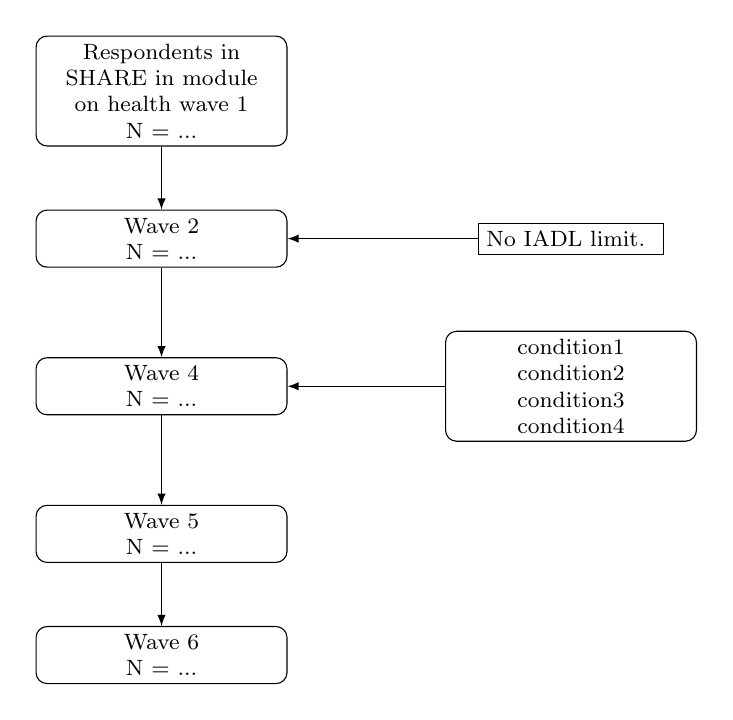
\begin{tikzpicture}
\footnotesize
\matrix (m)[matrix of nodes, column  sep=2cm, row  sep=8mm, align=center, nodes={rectangle,draw, anchor=center} ]{
|[block]| {Respondents in SHARE in module on health wave 1\\ N = ...} & \\
|[block]| {Wave 2 \\N = ...} & {No IADL limit.} \\
|[block]| {Wave 4 \\N = ...} & |[block]|{condition1 \\ condition2 \\ condition3 \\ condition4} \\
|[block]| {Wave 5\\N = ...} &  \\
|[block]| {Wave 6\\N = ...} &  \\
};

\path [>=latex,->] (m-1-1) edge (m-2-1);
\path [>=latex,->] (m-2-1) edge (m-3-1);
\path [>=latex,->] (m-3-1) edge (m-4-1);
\path [>=latex,->] (m-4-1) edge (m-5-1);
\path [>=latex,->] (m-2-2) edge (m-2-1);
\path [>=latex,->] (m-3-2) edge (m-3-1);

\end{tikzpicture}

Since there is no duration measure available in the SHARE data recording the age at onset of the IADL limitations, I construct the duration variable myself. If an individual reports to have a chronic disability in a particular wave, but not in the closest recorded preceding wave, the duration is calculated as the time in years between these two waves divided by two. If the individual has already reported chronic limitations for more than one wave, the full length in years between the current and preceding wave is added to the previously recorded duration. The time in years between two consecutive waves is based on the difference in age of a respondent between those waves. In the main model specification, duration is split up in dummy variables. The dummy variables indicate whether the onset of the chronic disability is reported within the past 2 years, between 2 and 5.5 years or more than 5.5 years ago. This division was chosen in order to spread out the subjects as much as possible across all dummy groups. 

Additionally, I control for sociodemographic characteristics, like gender, marital status (married or registered partnership, not married), employment status (retired, employed, unemployed, inactive), education (less than high school equivalent, high school equivalent, more than high school equivalent) and number of children. The reference categories for martial status, employment status and education are being married, being employed and high school education respectively.    

In table \ref{desc} it is apparent that by the end of data collection, about half of the observations concern individuals with disabilities. An overwhelming majority of the observations concerns individuals with a chronic illness. Considering that this measure also includes minor health impairments like hypertension and high blood pressure and the relatively older sample, this is not that surprising. The average number of limitations with IADL is 2.4. The average duration of having chronic limitations is 2 years. Note that relatively little observations fall into the categories Very good and Excellent for self-perceived health. This could be due to the age group studied in this data set, which is older compared to the general population with a mean age of 72. Moreover, approximately 41 \% is male and 62 \% is married. The majority of the sample is retired and about half of the sample does not have the equivalent of a modern high school degree. 
%The first wave consists of 30451 individuals, which expands to 68231 subjects in the last wave. The total number of subjects and observations is given in table \ref{table:descriptives1}. Individual retention from wave 1 to wave 2 lies around 69\%. From wave 2 to wave 4 this is 51\%, which might be due to relatively more attrition in this longer interim. The retention rates between wave 4 and 5, and 5 and 6, is approximately 67\%. 

\begin{table}[h!]
\centering
\footnotesize
\caption{Descriptive statistics}
\label{desc}
\begin{tabular}{l llll}
\hline
Variable                     & Definition   & Label & Mean & Standard \\
                             &              &       &      & deviation\\\hline\hline
Life satisfaction$^{1}$      & 1 = Rating scale 1,2,3           & Life satisfaction 1   & 0.049 & 0.216 \\
                             & 2 = Rating scale 4               & Life satisfaction 2   & 0.030 & 0.171 \\
                             & 3 = Rating scale 5               & Life satisfaction 3   & 0.159 & 0.365 \\
                             & 4 = Rating scale 6               & Life satisfaction 4   & 0.102 & 0.303 \\
                             & 5 = Rating scale 7               & Life satisfaction 5   & 0.171 & 0.377 \\
                             & 6 = Rating scale 8               & Life satisfaction 6   & 0.256 & 0.437 \\
                             & 7 = Rating scale 9               & Life satisfaction 7   & 0.107 & 0.309 \\
                             & 8 = Rating scale 10              & Life satisfaction 8   & 0.126 & 0.332 \\
Self-perceived health        & 1 = Poor                         & Poor                  & 0.263 & 0.440 \\
                             & 2 = Fair                         & Fair                  & 0.421 & 0.494 \\
                             & 3 = Good                         & Good                  & 0.243 & 0.429 \\
                             & 4 = Very good                    & Very good             & 0.056 & 0.230 \\
                             & 5 = Excellent                    & Excellent             & 0.017 & 0.130 \\
Incidence of disability      & Incidence of any number of       & Disability incidence  & 0.451 & 0.498 \\      
                             & chronic limitations with IADL    &                       &       &       \\ 
Incidence of chronic illness & Incidence of chronic illness     & Illness incidence     & 0.832 & 0.374 \\
Number of limitations$^{2}$  & Number of chronic limitations    & Number of limitations & 2.433 & 2.020 \\
                             & with IADL                        &                       &       &       \\
Duration$^{2}$               & Duration of chronic disability   & Disability duration   & 2.000 & 1.653 \\
Gender                       & 1 = Male                         & Male                  & 0.413 & 0.492 \\
Age                          & Age                              & Age                   &72.108 &10.388 \\
Martial status               & 1 = Married/                     & Married/              & 0.618 & 0.486 \\
                             & Registered partnership           & Registered partnership&       &       \\
Employment                   & 1 = Retired                      & Retired               & 0.712 & 0.453 \\
                             & 2 = Employed                     & Employed              & 0.087 & 0.283 \\
                             & 3 = Unemployed                   & Unemployed            & 0.023 & 0.149 \\
                             & 4 = Inactive                     & Inactive              & 0.178 & 0.383 \\
Education$^{3}$              & 1 =$<$ high school               & $<$ high school       & 0.544 & 0.498 \\
                             & 2 = High school                  & High school           & 0.210 & 0.407 \\
                             & 3 = $>$ high school              & $>$ high school       & 0.246 & 0.431 \\
Number of children           & Number of children               & Number of children    & 2.276 & 1.534 \\
Number of observations &&&\\
\hline
\end{tabular}
\caption*{\footnotesize{$^{1}$ Life satisfaction is measured on a scale from 1 to 11 where 1 means completely dissatisfied and 11 means completely satisfied. The first three rating scale categories were merged in order to fill the first category enough for estimation purposes.\\
$^{2}$ Number of limitations and duration are calculated taking only the observations with a chronic disability into account.\\
$^{3}$ Education is measured by transforming the years of education in terms of high school duration. \\}}
\end{table} 
\textcolor{red}{education eruit}
\textcolor{red}{WOPPING GRAPH}

\FloatBarrier

%%%%%%%%%%%%%%%%%%%%%%%%%%%%%%%%%%%%%%%%%%%%%%%%%%%%%%%%%%%%%%%%%%%%%%%%%%%%%%%%%%%%%%%%%%%%%%%%%%%%%%%%%%%%%%%%%%%%%%%%%%%%%%%%%%%%%%%%%%%%%%%%
\clearpage

\subsection{Results fixed effects ordered logit model}

Here, I present the results for the estimation of the fixed effects ordered logit model. Table \ref{logit} presents the regression estimates for both the analysis with life satisfaction and that with self-perceived health. 

In the regression with life satisfaction...\textcolor{red}{significance covariates} The estimated coefficient on the number of IADL limitations is significant and negative. This can be seen as evidence that a higher number of limitations is related to a lower life satisfaction. Moreover, there is no significant difference in the effect of no limitations with respect to 0 to 2 years of limitations on life satisfaction. Furthermore, the coefficient on more than 5.5 years of IADL limitations is significant and positive. This supports the adaptation hypothesis, meaning that higher levels of life satisfaction are more prevalent amongst individuals who have lived with chronic disability longer.   

In the regression with self-perceived health... The number of IADL limitations also has a significant negative effect on self-perceived health. Interestingly, there is significant difference in the effect of a duration of 0 to 2 years and that of no limitations on self-perceived health. The positive sign indicates that individuals with no IALD limitations have a higher self-perceived health than those that have recently experienced the onset of disability. There is no indication of adaptation, with the subsequent duration dummies of 2 to 5.5 years and more than 5.5 years not being significantly different from 0 to 2 years. 

\textcolor{blue}{education, number of children misschien eruit}

\begin{table}[htbp]
\centering
\footnotesize
\caption{FE ordered logit regression}
\label{logit}
\begin{tabular}{ll ll}
\hline
& & Life satisfaction & Self-perceived\\
& &                    &health\\\hline\hline
\multicolumn{2}{l}{\textbf{Marital status}}\\
\multicolumn{2}{l}{(Ref. Married)}\\
& Not married                           & -0.254         & -0.048           \\
&                                       &  (0.157)       &  (0.152)         \\
\multicolumn{2}{l}{\textbf{Employment status}}\\
\multicolumn{2}{l}{(Ref. Employed)}\\
&Retired                  & -$0.443^{***}$ & -$0.725^{***}$   \\
&                              &  (0.133)       &  (0.146)         \\
&Unemployed               & -$0.705^{**}$  & -$0.662^{**}$    \\
&                             &  (0.235)       &  (0.228)         \\
&Inactive                 & -$0.555^{***}$ & -$0.824^{***}$   \\
&                             &  (0.142)       &  (0.148)         \\
\multicolumn{2}{l}{\textbf{Number of children}}\\
&Number of children       &  0.046         & -0.029           \\
&                                        &  (0.038)       &  (0.027)         \\
\multicolumn{2}{l}{\textbf{Duration}}\\
\multicolumn{2}{l}{(Ref. 0-2 years IADL limitations)}\\
& 0 years IADL limit.      &  0.028         &  $0.929^{***}$   \\
&                 &  (0.118)       &  (0.204)         \\
&2-5.5 years IADL limit.  &  0.141         & -0.044           \\
&                &  (0.075)       &  (0.080)         \\
&$>$ 5.5 years IADL limit.&  $0.474^{***}$ & -0.026           \\
&               &  (0.144)       &  (0.146)         \\
\multicolumn{2}{l}{\textbf{Number of IADL limitations}}\\
& Number of IADL limit.    & -$0.157^{***}$ & -$0.163^{***}$   \\
&                                        &  (0.029)       &  (0.027)         \\
\multicolumn{2}{l}{Number of subjects}       &   5259         &  5341            \\
\multicolumn{2}{l}{Number of observations}   &   13328        &  15802           \\
\hline
\end{tabular}
\caption*{\footnotesize{\textit{Note}. The significant codes are as follows: *** indicates $p < 0.001$, ** indicates $p < 0.01$, * indicates $p <0.05$. Standard errors are reported underneath the regression estimates within parentheses. Standard errors are obtained by means of a cluster robust variance estimation.}}
\end{table}

%sphus            Estimate Std. Error     z value     Pr(>|t|) star
%mstatd1      -0.04751326 0.15150577 -0.31360694 7.538196e-01     
%employmentd1 -0.72470948 0.14618855 -4.95736126 7.145704e-07  ***
%employmentd2 -0.66211254 0.22816732 -2.90187277 3.709392e-03   **
%employmentd3 -0.82448004 0.14773011 -5.58098857 2.391554e-08  ***
%iscedd1       0.23050557 0.12731791  1.81047242 7.022256e-02     
%iscedd2      -0.01019081 0.12208679 -0.08347181 9.334764e-01     
%child        -0.02867040 0.02679181 -1.07011791 2.845662e-01     
%0             0.92919713 0.20431519  4.54786118 5.419386e-06  ***
%5.5          -0.04395088 0.07989773 -0.55008916 5.822582e-01     
%>5.5         -0.02587633 0.14629281 -0.17688041 8.596023e-01     
%IADL         -0.16324327 0.02698471 -6.04947303 1.453204e-09  ***

%lifesat         Estimate Std. Error    z value     Pr(>|t|) star
%mstatd1      -0.25449342 0.15736424 -1.6172253 1.058297e-01     
%employmentd1 -0.44277215 0.13283555 -3.3332352 8.584234e-04  ***
%employmentd2 -0.70461476 0.23514463 -2.9965164 2.730835e-03   **
%employmentd3 -0.55522075 0.14170198 -3.9182287 8.920206e-05  ***
%iscedd1       0.16654501 0.18185054  0.9158346 3.597537e-01     
%iscedd2       0.17400887 0.17983201  0.9676190 3.332347e-01     
%child         0.04614796 0.03788008  1.2182647 2.231234e-01     
%0             0.02812696 0.11771473  0.2389417 8.111508e-01     
%5.5           0.14137398 0.07488526  1.8878747 5.904278e-02     
%>5.5          0.47418029 0.14385088  3.2963322 9.795611e-04  ***
%IADL         -0.15684048 0.02879898 -5.4460432 5.150262e-08  ***

Table \ref{marginallifesat} and \ref{marginalsphus} present the estimated marginal effects for the regression with life satisfaction and self-perceived health respectively. The effects represent the size of the effect of a marginal increase in a regressor on the probability of falling into a category higher than $k$. 

From the table for life satisfaction, it is apparent that a unit increase in the number of IADL limitations, decreases the probability of reporting higher than categories 1, 2, 3, 4, 5, 6, 7 and 8 with approximately 0.8, 1.3, 3.2, 3.9, 4.4, 3.1 and 1.9 percentage points. On the other hand, having experienced a chronic disability for over 5.5 years increases the probability of reporting a life satisfaction category higher than 1, 2, 3, 4, 5, 6 or 7 by 2.3, 3.5, 8.8, 10.9, 12.2, 8.7 and 5.4 percentage points respectively.  

\begin{table}[htbp]
\centering
\footnotesize
\caption{Marginal effects on the probability of reporting Y$>$k}
\label{marginallifesat}
\begin{tabular}{ll llllllll}
\hline
& \multicolumn{7}{c}{Life satisfaction}\\
&          & Score 1 & Score 2 & Score 3 & Score 4 & Score 5 & Score 6 & Score 7 & Score 8\\
&          & \multicolumn{2}{l}{Very dissatisfied} & & & & &\multicolumn{2}{r}{Very satisfied}\\\hline\hline
\multicolumn{2}{l}{\textbf{Duration}} \\
\multicolumn{8}{l}{(Ref. 0-2 years IADL limitations)}\\
            & 0 years (NO) & -0.001 & -0.001 & -0.003 & -0.004 & -0.004 & -0.003 & -0.002 & - \\
            & IADL limit.  &&&&&&& \\
            & 2-5.5 years  &  0.007 &  0.010 &  0.026 &  0.032 &  0.036 &  0.026 &  0.016 & - \\
            & IADL limit.  &&&&&&& \\
            & $>$ 5.5 years&  0.023 &  0.035 &  0.088 &  0.109 &  0.122 &  0.087 &  0.054 & - \\
            & IADL limit.  &&&&&&& \\
\multicolumn{8}{l}{\textbf{Number of IADL limitations}}\\            
            & Number of    & -0.008 & -0.013 & -0.032 & -0.039 & -0.044 & -0.031 & -0.019 & - \\
            & IADL limit.  &&&&&&& \\
\hline
\end{tabular}
\caption*{\footnotesize{\textit{Note}. The marginal effects for the covariates are not shown for paucity. The covariates included are marital status, employment status, education and number of children. The reference categories are married, employed and high school education.}}
\end{table}

The marginal effects for the regression with self-perceived health show that the number of IADL limitations decreases the probability of reporting higher than the categories Poor, Fair, Good and Very good by 3.3, 3.6, 1.1 and 0.3 percentage points respectively. Moreover, not having any IADL limitations with respect to having chronic disability for 0 to 2 years increases the likelihood of reporting a category higher than Poor, Fair, Good an Very good with 17.3, 19.3, 6.1 and 1.5 percentage points. Note that the effect is a lot smaller for the categories Good and Very good, which might be counterintuitive, since this effect concerns people who do not have any disabilities. However, this could be due to the fact that the proportion of individuals reporting a self-perceived health that is Very good or Excellent is very small (see table \ref{distsphus}). 

\begin{table}[htbp]
\centering
\footnotesize
\caption{Marginal effects on the probability of reporting Y$>$k}
\label{marginalsphus}
\begin{tabular}{ll lllll}
\hline
&& \multicolumn{4}{c}{Self-perceived health}\\
&& Poor & Fair & Good & Very good & Excellent \\\\\hline\hline
\multicolumn{2}{l}{\textbf{Duration}} \\
\multicolumn{2}{l}{(Ref. 0-2 years IADL limitations)}\\
& years IADL limit.      &  0.173 &  0.193 &  0.061 &  0.015 & - \\
                 &&&& \\
& 2-5.5 years IADL limit.  & -0.008 & -0.009 & -0.003 & -0.001 & - \\
                &&&& \\
& $>$ 5.5 years IADL limit.& -0.005 & -0.006 & -0.002 & -0.000 & - \\
                 &&&& \\
\multicolumn{2}{l}{\textbf{Number of IADL limitations}}\\   
& Number of IADL limit.    & -0.033 & -0.036 & -0.011 & -0.003 & - \\
                                        &&&& \\
\hline
\end{tabular}
\caption*{\footnotesize{\textit{Note}. Ref. stands for reference category. The marginal effects for the covariates are not shown for paucity. The covariates included are marital status, employment status, education and number of children. The reference categories are married, employed and high school education.}}
\end{table}

\FloatBarrier

%%%%%%%%%%%%%%%%%%%%%%%%%%%%%%%%%%%%%%%%%%%%%%%%%%%%%%%%%%%%%%%%%%%%%%%%%%%%%%%%%%%%%%%%%%%%%%%%%%%%%%%%%%%%%%%%%%%%%%%%%%%%%%%%%%%%%%%%%%%%%%%%

\subsection{Results OLS and probit models}

\FloatBarrier

%%%%%%%%%%%%%%%%%%%%%%%%%%%%%%%%%%%%%%%%%%%%%%%%%%%%%%%%%%%%%%%%%%%%%%%%%%%%%%%%%%%%%%%%%%%%%%%%%%%%%%%%%%%%%%%%%%%%%%%%%%%%%%%%%%%%%%%%%%%%%%%%

\subsubsection{Results fixed effects OLS model}

Table \ref{OLS} presents the regression estimates for the fixed effects linear OLS model.\\
For the full table of results including the effects of covariates see appendix A.3. 

\begin{table}[htbp]
\centering
\footnotesize
\caption{FE linear least squares}
\label{OLS}
\begin{tabular}{l ll}
\hline
Variable & Life satisfaction & Self-perceived \\
(Reference category)&        &  health\\\hline\hline
0 years (NO) IADL limit.                &  0.041         &  $0.319^{***}$   \\
(0-2 years IADL limit.)                 &  (0.042)       &  (0.017)         \\
\rule{0pt}{3ex}2-5.5 years IADL limit.  &  $0.114^{*}$   &  0.019           \\
(0-2 years IADL limitations)            &  (0.053)       &  (0.024)         \\
\rule{0pt}{3ex}$>$ 5.5 years IADL limit.&  $0.363^{***}$ &  0.049           \\
(0-2 years IADL limitations)            &  (0.103)       &  (0.043)         \\
\rule{0pt}{3ex}Number of IADL limit.    & -$0.164^{***}$ & -$0.082^{***}$   \\
                                        &  (0.015)       &  (0.005)         \\
\rule{0pt}{3ex}Number of subjects       & 5259           & 5341             \\
Number of observations                  & 13328          & 15802            \\
\hline
\end{tabular}
\caption*{\footnotesize{\textit{Note}. The significant codes are as follows: *** indicates $p < 0.001$, ** indicates $p < 0.01$, * indicates $p <0.05$. Standard errors are reported underneath the regression estimates within parentheses. The regression estimates for the covariates are not shown for paucity. The covariates included are marital status, employment status, education and number of children. The reference categories are married, employed and high school education.}}
\end{table}

\FloatBarrier

%%%%%%%%%%%%%%%%%%%%%%%%%%%%%%%%%%%%%%%%%%%%%%%%%%%%%%%%%%%%%%%%%%%%%%%%%%%%%%%%%%%%%%%%%%%%%%%%%%%%%%%%%%%%%%%%%%%%%%%%%%%%%%%%%%%%%%%%%%%%%%%%

\subsubsection{Results fixed effects ordered probit model}

Table \ref{probit} presents the regression estimates for the fixed effects ordered probit model.\\
For the full table of results including the effects of covariates see appendix A.4. 
\textcolor{red}{explain reference category for response variable according to paper}
\begin{table}[htbp]
\centering
\footnotesize
\caption{Ordered probit model life satisfaction}
\label{probit}
\begin{tabular}{ll ll}
\hline
\multicolumn{2}{c}{Life satisfaction} & \multicolumn{2}{c}{Self-perceived health}\\
Variable & Coefficients & Variable & Coefficients\\
(Reference category) & & (Reference category) & \\\hline\hline
$Y_{t-1}$ = 2               &  0.693            & $Y_{t-1}$ = Fair            &  $0.589^{***}$ \\
($Y_{t-1}$ = 1)             &  (0.36)           & ($Y_{t-1}$ = Poor)          &  (0.068)        \\
$Y_{t-1}$ = 3               &  $0.852^{*}$      & $Y_{t-1}$ = Good            &  $0.970^{***}$\\
($Y_{t-1}$ = 1)             &  (0.415)          & ($Y_{t-1}$ = Poor)          &  (0.098)        \\
$Y_{t-1}$ = 4               &  $0.932^{*}$      & $Y_{t-1}$ = Very good       &  $1.241^{***}$  \\
($Y_{t-1}$ = 1)             &  (0.422)          & ($Y_{t-1}$ = Poor)          &  (0.145)        \\
$Y_{t-1}$ = 5               &  $1.162^{**}$     & $Y_{t-1}$ = Excellent       &  $1.330^{***}$  \\
($Y_{t-1}$ = 1)             &  (0.385)          & ($Y_{t-1}$ = Poor)          &  (0.346)\\
$Y_{t-1}$ = 6               &  $1.380^{***}$&&\\
($Y_{t-1}$ = 1)             &  (0.354)      &&\\
$Y_{t-1}$ = 7               &  $1.549^{***}$&&\\
($Y_{t-1}$ = 1)             &  (0.336)      &&\\
$Y_{t-1}$ = 8               &  $1.748^{***}$&&\\
($Y_{t-1}$ = 1)             &  (0.373)      &&\\
$Y_{t,1}$ = 2               &  0.720            & $Y_{t,1}$ = Fair            &  0.258\\
($Y_{t,1}$ = 1)             &  (0.448)          & ($Y_{t,1}$ = Poor)          &  (0.144)\\
$Y_{t,1}$ = 3               &  0.728            & $Y_{t,1}$ = Good            &  $0.508^{**}$\\
($Y_{t,1}$ = 1)             &  (0.490)          & ($Y_{t,1}$ = Poor)          &  (0.173)\\
$Y_{t,1}$ = 4               & $0.888^{*}$       & $Y_{t,1}$ = Very good       &  $0.713^{**}$\\
($Y_{t,1}$ = 1)             &  (0.432)          & ($Y_{t,1}$ = Poor)          &  (0.227)\\
$Y_{t,1}$ = 5               &  $0.861^{*}$      & $Y_{t,1}$ = Excellent       &  $1.050^{**}$\\
($Y_{t,1}$ = 1)             &  (0.435)          & ($Y_{t,1}$ = Poor)          &  (0.380)\\
$Y_{t,1}$ = 6               &  $1.061^{*}$ &&\\
($Y_{t,1}$ = 1)             &  (0.461)     &&\\
$Y_{t,1}$ = 7               &  $1.226^{**}$&&\\
($Y_{t,1}$ = 1)             &  (0.445)      &&\\
$Y_{t,1}$ = 8               &  $1.248^{*}$  &&\\
($Y_{t,1}$ = 1)             &  (0.506)      &&\\
Disability duration         &  $0.100^{**}$     & Disability duration         &  $0.042^{*}$\\
                            &  (0.031)          &                             &  (0.018)\\
Incidence disability        & -0.127            & Incidence disability        & -$0.455^{***}$\\
                            &  (0.121)          &                             & (0.042)\\
Number of IADL limitations  & -$0.061^{*}$      & Number of IADL limitations  & -$0.121^{***}$\\
                            &  (0.024)          &                             & (0.019)\\
Threshold 1                 &  0.946            & Threshold 1                 & 0.040          \\
Threshold 2                 &  1.215            & Threshold 2                 & 1.468          \\
Threshold 3                 &  2.006            & Threshold 3                 & 2.683          \\
Threshold 4                 &  2.344            & Threshold 4                 & 3.504          \\
Threshold 5                 &  2.841            &                             &\\
Threshold 6                 &  3.658            &                             &\\
Threshold 7                 &  4.133            &                             &\\
Number of subjects          &  4556             & Number of subjects          & 5335\\
Number of observations      &  8252             & Number of observations      & 10455\\
\hline
\end{tabular}
\caption*{\footnotesize{\textit{Note}. The significant codes are as follows: *** indicates $p < 0.001$, ** indicates $p < 0.01$, * indicates $p <0.05$. Standard errors are reported underneath the regression estimates within parentheses. Standard errors are obtained via the inverse of the negative hessian calculated with a maximum likelihood approach at the optimized estimates. The regression estimates for the covariates are not shown for paucity. The covariates included are marital status, employment status, education and number of children. The reference categories are married, employed and high school education.}}
\end{table}

\FloatBarrier

%%%%%%%%%%%%%%%%%%%%%%%%%%%%%%%%%%%%%%%%%%%%%%%%%%%%%%%%%%%%%%%%%%%%%%%%%%%%%%%%%%%%%%%%%%%%%%%%%%%%%%%%%%%%%%%%%%%%%%%%%%%%%%%%%%%%%%%%%%%%%%%%

\subsection{Robustness checks}

The first two columns of table \ref{robust1} present the regression estimates for the fixed effects ordered logit model applied to individuals whose limitations with IADL stay constant over their entire observed period.\\
The second two columns of table \ref{robust1} present the regression estimates for the fixed effects ordered logit model applied to individuals whose limitations with IADL increase over their observed period.\\
Table \ref{robust2} presents the regression estimates for the fixed effects ordered logit model where duration is continuous as opposed to divided into dummy variables.\\
Table \ref{robust3} presents the regression estimates for the fixed effects ordered logit model applied to individuals who are observed for at least three waves.\\

\begin{table}[htbp]
\centering
\footnotesize
\caption{FE ordered logit regression continuous duration}
\label{robust2}
\begin{tabular}{l ll}
\hline
Variable & Life satisfaction & Self-perceived \\
(Reference category) &  & health\\\hline\hline
\rule{0pt}{3ex}Disability duration      &  $0.053^{*}$   & -$0.129^{*}$     \\
                                        &  (0.024)       &  (0.053)         \\
\rule{0pt}{3ex}Number of IADL limit.    & -$0.170^{***}$ & -$0.267^{***}$   \\
                                        &  (0.021)       &  (0.028)         \\
\rule{0pt}{3ex}Number of subjects       &  5259          &  5341            \\
Number of observations                  &  13328         &  15802           \\
\hline
\end{tabular}
\caption*{\footnotesize{\textit{Note}. The significant codes are as follows: *** indicates $p < 0.001$, ** indicates $p < 0.01$, * indicates $p <0.05$. Standard errors are reported underneath the regression estimates within parentheses. The regression estimates for the covariates are not shown for paucity. The covariates included are marital status, employment status, education and number of children. The reference categories are married, employed and high school education.}}
\end{table}
% continuous duration
%lifesat         Estimate Std. Error    z value     Pr(>|t|) star
%mstatd1      -0.28040527 0.16349368 -1.7150832 8.632997e-02     
%employmentd1 -0.49707202 0.14133068 -3.5170849 4.363141e-04  ***
%employmentd2 -0.73231289 0.22399446 -3.2693349 1.078006e-03   **
%employmentd3 -0.60198042 0.14441966 -4.1682720 3.069175e-05  ***
%iscedd1       0.15773710 0.18242980  0.8646455 3.872334e-01     
%iscedd2       0.16995608 0.17386097  0.9775401 3.283018e-01     
%child         0.04169294 0.03705573  1.1251417 2.605290e-01     
%dur2          0.05302100 0.02402862  2.2065771 2.734362e-02    *
%IADL         -0.17002009 0.02141562 -7.9390684 2.037055e-15  ***
%sphus           Estimate Std. Error    z value     Pr(>|t|) star
%mstatd1      -0.12306426 0.16390447 -0.7508292 4.527554e-01     
%employmentd1 -0.88337014 0.15043204 -5.8722205 4.299962e-09  ***
%employmentd2 -0.63399636 0.21862525 -2.8999229 3.732545e-03   **
%employmentd3 -0.92760074 0.15134673 -6.1289778 8.844548e-10  ***
%iscedd1       0.26280271 0.12668905  2.0743917 3.804295e-02    *
%iscedd2       0.01090945 0.12031797  0.0906718 9.277534e-01     
%child        -0.02872661 0.02710324 -1.0598958 2.891920e-01     
%dur2         -0.12918952 0.05255651 -2.4581070 1.396715e-02    *
%IADL         -0.26678789 0.02826809 -9.4377762 3.807748e-21  ***


\FloatBarrier

\section{Discussion}

\subsection{Summary}
I analyzed adaptation with a fixed effects ordered logit model making use of the BUC estimator proposed by Baetschmann, Staub and Winkelmann (2015). Supportive evidence for adaptation in the life satisfaction data was found, but not in self-perceived health. 

The obvious discrepancy between these two results might first of all be due to the nature of the dependent variables. It is likely that people take many factors into account when answering a question about life satisfaction, which makes it into a more holistic measure of well-being. Hence, adaptation to chronic infirmity might be more apparent on the life satisfaction scale, since other factors like social support also affect this measure over time. In contrast, self-reported health is a much more narrowly defined construct, which presumably focuses people's attention on their health situation, which is not likely to have improved due to its chronic nature. \textcolor{red}{life satisfaction is hardly affected by chronic disability --> happy people stay happy, sad people stay sad}

Considering the replication results of the study by Clark, D'Ambrosio and Ghislandi, I find that there could indeed be adaptation to chronic illness, although my results do not provide sufficient evidence. The coefficients on the duration dummies become increasingly less negatively related to good health and in some model specifications even positive. Hence, it might be worthwhile to study the effect of longer duration spells and see whether this observed trend develops into fully observable adaptation.

I do not find the significant effect of duration on self-reported health that Cub\'i-Moll\`a, Jofre-Boner and Serra-Sastre find.  

\subsection{Limitations}
A limitation of this study is that its prospective nature (I can only include individuals whose onset of chronic infirmity is known) severely limits the effect of duration I can measure. My maximum duration time is 9.5 years and only a very small chronically indisposed sub-sample is observed for that period. Taking into account that  Cub\'i-Moll\`a, Jofre-Bonet, and Serra-Sastre (2016) only found a significant effect of duration after 20 years, the observed period in the SHARE data might simply not be long enough. Hence, future research should pay attention to the time scope of their data before conducting the analysis.

Furthermore, the SHARE data set is restricted to individuals of age 50 and up. It is possible that the adaptation process of the SHARE subjects differs from that of younger individuals. For example, it is imaginable that younger subjects find it easier to adapt to a chronic disability or disease, since they can more easily change their occupation or are less reliant on social support. Thus, the differences in the adaptation process for different age categories is a question for future research. Alternatively, the chronic conditions prevalent in the younger sample might be different to those reported by the older sample and the adaptation process for these subsets of diseases could differ.

Finally, a disadvantage of the methodology of Cub\'i-Moll\`a, Jofre-Boner and Serra-Sastre is that it heavily relies on the correct parameterization of the individual specific effects. It is true that this approach notably simplifies the analysis, but if the parameterization is misspecified the estimations will be inconsistent. 

\subsection{Implicication theory}
\textcolor{red}{kortere termijn adaptatie?}
\subsection{Implications practice}
\textcolor{red}{health state preferences}
\subsection{conclusions}
In conclusion, the different results for the adaptation analyses with life satisfaction and self-perceived health indicate that the adaptation response shift process differs depending on the construct used, a testament to the fact that happy people might not have the best of everything, but make the best of everything. 

\addcontentsline{toc}{section}{REFERENCES}
\section*{\centering REFERENCES}

\noindent Baetschmann, G., Staub, K.E. \& Winkelmann, R. (2015). Consistent estimation of the fixed effects ordered logit model. \textit{Journal of the Royal Statistical Society, A, 178(3),} 685-703.\\

\noindent Brickman, P., Coates, D. \& Janoff-Bulman, R. (1978). Lottery winners and accident victims: Is happiness relative? \textit{Journal of Personality and Social Psychology, 36}, 917–927.\\

\noindent Börsch-Supan, A., Brandt, M., Hunkler, C., Kneip, T., Korbmacher, J., Malter, F., Schaan, B., Stuck, S., Zuber, S.; SHARE Central Coordination Team. (2013). Data resource profile: The Survey of Health, Ageing and Retirement in Europe (SHARE). \textit{Int J Epidemiol., 42(4),} 992-1001. \\

\noindent Clark, A.E., D’Ambrosio, C. \& Ghislandi, S. (2016). Adaptation to poverty in long-run panel data. \textit{Review of Economics and Statistics, 98(3),} 591-600.\\

\noindent Cub\'i-Moll\`a, P., Jofre-Bonet, M. \& Serra-Sastre, V. (2016). Adaptation to health states: Sick yet better off? \textit{Health Economics,} 1-18.\\

\noindent Frederick, S. \& Loewenstein, G. (1999). \textit{Hedonic adaptation.} In: Diener, E., Schwarz, N. \& Kahneman, D. (Eds.), Hedonic Psychology: Scientific Approaches to Enjoyment, Suffering, and Well-Being. Russell Sage Foundation, New York, pp. 302–329.\\

\noindent Greene, W. (2004). The behaviour of the maximum likelihood estimator of limited
dependent variable models in the presence of fixed effects. \textit{Econometrics Journal, Vol 7(1)}, 98-119.\\

\noindent Krahn, M., Ritvo, P., Irvine, J., Tomlinson, G., Bremmer, K.E., Bezjak, A., Trachtenberg, J. \& Naglie, G. (2003). Patient and community preferences for outcomes in prostate cancer: Implications for clinical policy. \textit{Medical Care, 41(1),} 153-164.\\ 

\noindent Lucas, R.E. (2007). Long-term disability is associated with lasting changes in subjective well-being: Evidence from two nationally representative longitudinal studies. \textit{Journal of Personality and Social Psychology, 92,} 717–730.\\

\noindent Menzel, P., Dolan, P., Richardson, J. \& Olsen, J.A. (2002). The role of adaptation to disability and disease in health state valuation: A preliminary normative analysis. \textit{Social Science \& Medicine, 55,} 2149-2158.\\

\noindent Neyman, J. \& Scott E.L. (1948). Consistent Estimates Based on Partially Consistent Observations. \textit{Econometrica, 16(1),} 1-32.\\

\noindent Oswald, A.J. \& Powdthavee, N. (2008). Does happiness adapt? A longitudinal study of disability with implications for economists and judges. \textit{Journal of Public Economics, 92,} 1061-1077.\\

\noindent Peeters, Y. \& Stiggelbout, A.M. (2010). Health state valuations of patients and the general public analytically compared: A meta-analytical comparison of patient and population health state utilities. \textit{Value in Health, 13(2),} 306-309.\\ 

\noindent Sackett, D.L. \& Torrance, G.W. (1978). The utility of different health states as perceived by the general public. \textit{Journal of Chronic Diseases, 32(11),} 697-704.\\

\noindent Schulz, R. \& Decker, S. (1985). Long-term adjustment to physical disability: The role of social support, perceived control, and self-blame. \textit{Journal of Personality and Social Psychology, 48(5),} 1162-1172.\\ 

\noindent Sprangers, M.A.G. \& Schwartz, C.E. (1999). Integrating response shift into health-related quality of life research: A theoretical model. \textit{Social Science \& Medicine 48,} 1507-1515.\\

\begin{sloppypar}
    \noindent Survey of Health, Ageing and Retirement in Europe. (2017, March 31). Release Guide 6.0.0. Retrieved from: 
    \url{http://www.share-project.org/fileadmin/pdf_documentation/SHARE_release_guide_6-0-0.pdf}.\\
\end{sloppypar}

\noindent Tyc, V. L. (1992). Psychosocial adaptation of children and adolescents with limb deficiencies: A review. \textit{Clinical Psychology Review, 2,} 275-91.\\

\noindent Versteegh, M.M. \& Brouwer, W.B.F. (2016). Patient and general public preferences for health states: A call to reconsider current guidelines. \textit{Social Science \& Medicine, 165,} 66-74.\\

\noindent Wooldridge, J.M. (2005). Simple solutions to the initial conditions problem in dynamic, nonlinear panel data models with unobserved heterogeneity. \textit{Journal of Applied Econometrics, 20,} 39-54.\\

\noindent Zorginstituut Nederland. (2016). Bijlage 2 in Richtlijn voor het uitvoeren van economische evaluaties in de gezondheidszorg. Zorginstituut Nederland, Diemen, The Netherlands.

%%%%%%%%%%%%%%%%%%%%%%%%%%%%%%%%%%%%%%%%%%%%%%%%%%%%%%%%%%%%%%%%%%%%%%%%%%%%%%%%%%%%%%%%%%%%%%%%%%%%%%%%%%%%%%%%%%%%%%%%%%%%%%%%%%%%%%%%%%%%%%%%%%%%%%%%%%%%%%%%%%%%%%%%%%%%%%
\newpage 

\addcontentsline{toc}{section}{APPENDIX}
\section*{\centering APPENDIX}
\addcontentsline{toc}{subsection}{A.1 \quad Derivatives of the conditional likelihood function}
\subsection*{A.1}
The first order derivatives of the conditional likelihood function for the Chamberlain estimator are as follows:

\[
    s_{i}^k=\frac{\partial log(P_{i}^k(b))}{\partial b} = x_{i}'\Bigg\{ d_{i}^k - \sum_{j \in B_{i}}{j\frac{exp(j'x_{i}b)}{\sum_{l \in B_{i}}{exp(l'x_{i}b)}}} \Bigg\}.
\]

\noindent The individual Hessians for this likelihood function are given by

\[
    \begin{split}
        H_{i}^k(b) = \frac{\partial^2 log(P_{i}^k(b))}{\partial b\partial b'} = - \sum_{j \in B_{i}}{\frac{exp(j'x_{i}b)}{\sum_{l \in B_{i}}{exp(l'x_{i}b)}}} \times \\
        \Bigg( x_{i}'j - \sum_{m \in B_{i}}{\frac{exp(m'x_{i}b)}{\sum_{l \in B_{i}}{exp(l'x_{i}b)}}m'x_{i}} \Bigg)\Bigg( x_{i}'j - \sum_{m \in B_{i}}{\frac{exp(m'x_{i}b)}{\sum_{l \in B_{i}}{exp(l'x_{i}b)}}m'x_{i}} \Bigg)'.
    \end{split}
\]

\FloatBarrier

%%%%%%%%%%%%%%%%%%%%%%%%%%%%%%%%%%%%%%%%%%%%%%%%%%%%%%%%%%%%%%%%%%%%%%%%%%%%%%%%%%%%%%%%%%%%%%%%%%%%%%%%%%%%%%%%%%%%%%%%%%%%%%%%%%%%%%%%%%%%%%%%%%%%%%%%%%%%%%%%%%%%%%%%%%%%%%

\clearpage

\addcontentsline{toc}{subsection}{A.2 \quad Marginal effects ordered logit model}
\subsection*{A.2}

\begin{table}[htbp]
\centering
\footnotesize
\caption{Marginal effects on the probability of reporting Y$>$k}
\label{table1}
\begin{tabular}{l lllllll}
\hline
& \multicolumn{7}{c}{Life satisfaction}\\
Variable & Score 1 & Score 2 & Score 3 & Score 4 & Score 5 & Score 6 & Score 7\\
(Reference category) &\\\hline\hline
Not married                             & -0.012 & -0.018 & -0.046 & -0.056 & -0.063 & -0.045 & -0.028 \\
(Married)                               &&&&&&& \\
\rule{0pt}{3ex}Retired                  & -0.022 & -0.034 & -0.086 & -0.106 & -0.118 & -0.084 & -0.052 \\
(Employed)                              &&&&&&& \\
\rule{0pt}{3ex}Unemployed               & -0.034 & -0.053 & -0.131 & -0.162 & -0.181 & -0.129 & -0.080 \\
(Employed)                              &&&&&&& \\
\rule{0pt}{3ex}Inactive                 & -0.026 & -0.041 & -0.101 & -0.125 & -0.139 & -0.100 & -0.061 \\
(Employed)                              &&&&&&& \\
\rule{0pt}{3ex}Educ $<$ high school     &  0.007 &  0.012 &  0.029 &  0.036 &  0.040 &  0.029 &  0.018 \\
(High school)                           &&&&&&& \\
\rule{0pt}{3ex}Educ $>$ high school     &  0.009 &  0.015 &  0.036 &  0.045 &  0.050 &  0.036 &  0.022 \\
(High school)                           &&&&&&& \\
\rule{0pt}{3ex}Number of children       &  0.002 &  0.003 &  0.008 &  0.010 &  0.011 &  0.008 &  0.005 \\
                                        &&&&&&& \\
\rule{0pt}{3ex}0 years IADL limit.      & -0.001 & -0.001 & -0.003 & -0.004 & -0.004 & -0.003 & -0.002 \\
(0-2 years IADL limit.)                 &&&&&&& \\
\rule{0pt}{3ex}2-5.5 years IADL limit.  &  0.007 &  0.010 &  0.026 &  0.032 &  0.036 &  0.026 &  0.016 \\
(0-2 years IADL limit.)                 &&&&&&& \\
\rule{0pt}{3ex}$>$ 5.5 years IADL limit.&  0.023 &  0.035 &  0.088 &  0.109 &  0.122 &  0.087 &  0.054 \\
(0-2 years IADL limit.)                 &&&&&&& \\
\rule{0pt}{3ex}Number of IADL limit.    & -0.008 & -0.013 & -0.032 & -0.039 & -0.044 & -0.031 & -0.019 \\
                                        &&&&&&& \\
\hline
\end{tabular}
\end{table}
%lifesat                 >1           >2           >3           >4           >5           >6           >7
%mstatd1      -0.0117163447 -0.018307748 -0.045629026 -0.056487377 -0.062924247 -0.044968655 -0.027755184
%employmentd1 -0.0219916127 -0.034363696 -0.085645812 -0.106026968 -0.118108993 -0.084406294 -0.052096559
%employmentd2 -0.0336206826 -0.052535071 -0.130934948 -0.162093571 -0.180564519 -0.129039979 -0.079644995
%employmentd3 -0.0259527116 -0.040553238 -0.101072218 -0.125124399 -0.139382622 -0.099609440 -0.061480120
%iscedd1       0.0074462202  0.011635329  0.028999127  0.035900057  0.039990954  0.028579434  0.017639564
%iscedd2       0.0092866266  0.014511115  0.036166546  0.044773109  0.049875111  0.035643122  0.021999355
%child         0.0021259859  0.003322027  0.008279601  0.010249900  0.011417901  0.008159774  0.005036309
%dur0         -0.0007465176 -0.001166495 -0.002907295 -0.003599145 -0.004009276 -0.002865219 -0.001768447
%dur25.5       0.0067063407  0.010479207  0.026117684  0.032332916  0.036017329  0.025739693  0.015886842
%dur5.5        0.0226741265  0.035430180  0.088303846  0.109317535  0.121774528  0.087025859  0.053713386
%IADL         -0.0081809694 -0.012783435 -0.031860591 -0.039442464 -0.043937026 -0.031399485 -0.019380132

\begin{table}[h!]
\centering
\footnotesize
\caption*{Marginal effects on the probability of reporting Y$>$k}
\label{table1}
\begin{tabular}{l llll}
\hline
& \multicolumn{4}{c}{Self-perceived health}\\
Variable & Poor & Fair & Good & Very good \\
(Reference category) &&&&\\\hline\hline
Not married                             & -0.009 & -0.010 & -0.003 & -0.001 \\
(Married)                               &&&& \\
\rule{0pt}{3ex}Retired                  & -0.142 & -0.158 & -0.050 & -0.012 \\
(Employed)                              &&&& \\
\rule{0pt}{3ex}Unemployed               & -0.125 & -0.139 & -0.044 & -0.011 \\
(Employed)                              &&&& \\
\rule{0pt}{3ex}Inactive                 & -0.158 & -0.176 & -0.055 & -0.014 \\
(Employed)                              &&&& \\
\rule{0pt}{3ex}Educ $<$ high school     &  0.044 &  0.049 &  0.015 &  0.004 \\
(High school)                           &&&& \\
\rule{0pt}{3ex}Educ $>$ high school     & -0.000 & -0.000 & -0.000 & -0.000 \\
(High school)                           &&&& \\
\rule{0pt}{3ex}Number of children       & -0.007 & -0.008 & -0.002 & -0.001 \\
                                        &&&& \\
\rule{0pt}{3ex}0 years IADL limit.      &  0.173 &  0.193 &  0.061 &  0.015 \\
(0-2 years IADL limit.)                 &&&& \\
\rule{0pt}{3ex}2-5.5 years IADL limit.  & -0.008 & -0.009 & -0.003 & -0.001 \\
(0-2 years IADL limit.)                 &&&& \\
\rule{0pt}{3ex}$>$ 5.5 years IADL limit.& -0.005 & -0.006 & -0.002 & -0.000 \\
(0-2 years IADL limit.)                 &&&& \\
\rule{0pt}{3ex}Number of IADL limit.    & -0.033 & -0.036 & -0.011 & -0.003 \\
                                        &&&& \\
\hline
\end{tabular}
\end{table}
%sphus                >Poor         >Fair         >Good    >Very good
%mstatd1      -0.0091080406 -0.0101607846 -3.199210e-03 -0.0007921521
%employmentd1 -0.1416978955 -0.1580759096 -4.977156e-02 -0.0123238671
%employmentd2 -0.1246752829 -0.1390857548 -4.379235e-02 -0.0108433623
%employmentd3 -0.1577809336 -0.1760178901 -5.542075e-02 -0.0137226545
%iscedd1       0.0435778803  0.0486147874  1.530678e-02  0.0037900916
%iscedd2      -0.0001826076 -0.0002037141 -6.414115e-05 -0.0000158819
%child        -0.0067714424 -0.0075541131 -2.378478e-03 -0.0005889315
%dur0          0.1726084371  0.1925592162  6.062893e-02  0.0150122444
%dur25.5      -0.0083627219 -0.0093293190 -2.937416e-03 -0.0007273296
%dur5.5       -0.0049551975 -0.0055279393 -1.740519e-03 -0.0004309676
%IADL         -0.0327146978 -0.0364959945 -1.149108e-02 -0.0028452899

\FloatBarrier

%%%%%%%%%%%%%%%%%%%%%%%%%%%%%%%%%%%%%%%%%%%%%%%%%%%%%%%%%%%%%%%%%%%%%%%%%%%%%%%%%%%%%%%%%%%%%%%%%%%%%%%%%%%%%%%%%%%%%%%%%%%%%%%%%%%%%%%%%%%%%%%%%%%%%%%%%%%%%%%%%%%%%%%%%%%%%%

\clearpage

\addcontentsline{toc}{subsection}{A.3 \quad Results ordinary least squares linear fixed effects}
\subsection*{A.3} 
\begin{table}[htbp]
\centering
\footnotesize
\caption*{Complete ordinary least squares linear fixed effects regression on both life satisfaction and self-perceived health}
\label{table1}
\begin{tabular}{l lllll}
\hline
Reference category & Variable & \multicolumn{2}{l}{Life satisfaction} & \multicolumn{2}{l}{Self-perceived} \\
&                    &                   &  &  \multicolumn{2}{l}{health} \\\hline\hline
Married                        & Not Married                    & -$0.026^{*}$  & (0.111)   & -0.030        & (0.044)   \\
Employed                       & Retired                        & -$0.299^{**}$ & (0.094)   & -$0.286^{***}$& (0.039)   \\
                               & Unemployed                     & -$0.468^{**}$ & (0.157)   & -$0.267^{***}$& (0.065)   \\
                               & Inactive                       & -$0.387^{***}$& (0.103)   & -$0.326^{***}$& (0.042)   \\
High school                    & Educ $<$ high school           &  0.114        & (0.122)   &  0.062        & (0.046)   \\
                               & Educ $>$ high school           &  0.148        & (0.123)   &  0.004        & (0.043)   \\
-                              & Number of children             &  0.038        & (0.038)   & -0.001        & (0.015)   \\
\textcolor{red}{adaptation} &&&&\\
0-2 years IADL limitations     & 0 years \textcolor{red}{(NO)} IADL limitations  &  0.041        & (0.042)   &  $0.319^{***}$& (0.017)   \\
                               & 2-5.5 years IADL limitations   &  $0.114^{*}$  & (0.053)   &  0.019        & (0.024)   \\
                               & $>$ 5.5 years IADL limitations &  $0.363^{***}$& (0.103)   &  0.049        & (0.043)   \\
-                              & Number of IADL limitations     & -$0.164^{***}$& (0.015)   & -$0.082^{***}$& (0.005)   \\
-                              & Number of subjects             & 5259          &           & 5341          &           \\
-                              & Number of observations         & 13328         &           & 15802         &           \\
\hline
\end{tabular}
\caption*{\footnotesize{\textit{Note}. The significant codes are as follows: *** indicates $p < 0.001$, ** indicates $p < 0.01$, * indicates $p <0.05$. Standard errors are reported underneath the regression estimates within parentheses.}}
\end{table}

%lifesat          Estimate Std. Error      z value     Pr(>|z|) star
%mstatd1      -0.26250494 0.11083806  -2.3683646 1.786692e-02    *
%employmentd1 -0.29916216 0.09397026  -3.1835834 1.454642e-03   **
%employmentd2 -0.46759691 0.15708290  -2.9767524 2.913192e-03   **
%employmentd3 -0.38715091 0.10328335  -3.7484347 1.779417e-04  ***
%iscedd1       0.11374358 0.12194644   0.9327339 3.509574e-01     
%iscedd2       0.14800918 0.12260768   1.2071771 2.273640e-01     
%child         0.03783769 0.03753738   1.0080004 3.134543e-01     
%dur0          0.04110955 0.04150850   0.9903888 3.219841e-01     
%dur25         0.11357489 0.05349899   2.1229352 3.375928e-02    *
%dur5          0.36315545 0.10342671   3.5112348 4.460302e-04  ***
%IADL         -0.16396572 0.01536743 -10.6696916 1.410939e-26  ***

%sphus            Estimate  Std. Error      z value     Pr(>|z|) star
%mstatd1      -0.0296647469 0.043555492  -0.68107937 4.958213e-01     
%employmentd1 -0.2855674815 0.039101616  -7.30321425 2.809732e-13  ***
%employmentd2 -0.2673579305 0.064545726  -4.14214770 3.440686e-05  ***
%employmentd3 -0.3261163034 0.042029720  -7.75918334 8.547801e-15  ***
%iscedd1       0.0621219042 0.045551740   1.36376578 1.726413e-01     
%iscedd2       0.0039896440 0.043115978   0.09253284 9.262747e-01     
%child        -0.0005545406 0.014927393  -0.03714920 9.703660e-01     
%dur0          0.3189442352 0.017217696  18.52421139 1.317189e-76  ***
%dur25         0.0191352948 0.023293284   0.82149409 4.113649e-01     
%dur5          0.0492248110 0.043192361   1.13966474 2.544260e-01     
%IADL         -0.0815679330 0.005497114 -14.83831806 8.280618e-50  ***

\FloatBarrier

%%%%%%%%%%%%%%%%%%%%%%%%%%%%%%%%%%%%%%%%%%%%%%%%%%%%%%%%%%%%%%%%%%%%%%%%%%%%%%%%%%%%%%%%%%%%%%%%%%%%%%%%%%%%%%%%%%%%%%%%%%%%%%%%%%%%%%%%%%%%%%%%%%%%%%%%%%%%%%%%%%%%%%%%%%%%%%

\clearpage

\addcontentsline{toc}{subsection}{A.4 \quad Results fixed effects ordered probit}
\subsection*{A.4}

\begin{table}[h!]
\centering
\footnotesize
\caption*{Complete fixed effects ordered probit regression on self-perceived health.}
\label{table1}
\begin{tabular}{ll l l l}
\hline
\multicolumn{5}{c}{Self-perceived health} \\\\
 & \multicolumn{1}{l}{Reference category} & \multicolumn{1}{l}{Coefficients} & \multicolumn{2}{l}{Parameterization of FE}\\\hline\hline
$Y_{t-1}$ = Fair            & $Y_{t-1}$ = Poor &  $0.589^{***}$ & $Y_{t,1}$ &  0.258\\
                            &                  & (0.068)        &           &  (0.144)\\
$Y_{t-1}$ = Good            & $Y_{t-1}$ = Poor & $0.970^{***}$  & $Y_{t,1}$ &  $0.508^{**}$\\
                            &                  & (0.098)        &           &  (0.173)\\
$Y_{t-1}$ = Very good       & $Y_{t-1}$ = Poor & $1.241^{***}$  & $Y_{t,1}$ &  $0.713^{**}$\\
                            &                  & (0.145)        &           &  (0.227)\\
$Y_{t-1}$ = Excellent       & $Y_{t-1}$ = Poor & $1.330^{***}$  & $Y_{t,1}$ &  $1.050^{**}$\\
                            &                  & (0.346)        &           &  (0.380)\\
Not married                 & Married          & 0.070          & Mean      &  0.018\\
                            &                  & (0.118)        &           &  (0.123)\\
Retired                     & Employed         & -0.026         & Mean      &  0.055\\
                            &                  & (0.116)        &           &  (0.227)\\
Unemployed                  & Employed         & 0.074          & Mean      &  0.017\\
                            &                  & (0.186)        &           &  (0.326)\\
Inactive                    & Employed         & -0.065         & Mean      &  0.014\\
                            &                  & (0.120)        &           &  (0.231)\\
Educ $<$ high school        & High school      & 0.081          & Mean      & -0.065\\
                            &                  & (0.106)        &           &  (0.120)\\
Educ $>$ high school        & High school      & -0.009         & Mean      & -0.092\\
                            &                  &  (0.096)       &           &  (0.118)\\
Number of children          &                  & -0.015         & Mean      &  0.038\\
                            &                  &  (0.040)       &           &  (0.041)\\
Disability duration         &                  &  $0.042^{*}$   & Mean      & -0.030\\
                            &                  &  (0.018)       &           &  (0.024)  \\
Incidence disability        &                  & -$0.455^{***}$ & Mean      &  0.115\\
                            &                  & (0.042)        &           &  (0.121)\\
Number of IADL limitations  &                  & -$0.121^{***}$ & Mean      & -0.049  \\
                            &                  & (0.019)        &           &  (0.017)\\
Threshold 1                 &                  & 0.040          &&\\
Threshold 2                 &                  & 1.468          &&\\
Threshold 3                 &                  & 2.683          &&\\
Threshold 4                 &                  & 3.504          &&\\
Number of subjects          &                  & 5335           &&\\
Number of observations      &                  & 10455          &&\\
\hline
\end{tabular}
\caption*{\footnotesize{\textit{Note}. The significant codes are as follows: *** indicates $p < 0.001$, ** indicates $p < 0.01$, * indicates $p <0.05$. Standard errors are reported underneath the regression estimates within parentheses. Standard errors are obtained via the inverse of the negative hessian calculated with a maximum likelihood approach at the optimized estimates.}}
\end{table}

%sphus                Estimate Std. Error      z value      Pr(>|t|) star
%lagd1             0.58948453 0.06778157   8.69682592 3.412964e-18  ***
%lagd2             0.97043980 0.09816960   9.88533923 4.819467e-23  ***
%lagd3             1.24061218 0.14471654   8.57270486 1.010823e-17  ***
%lagd4             1.33041396 0.34556578   3.84995859 1.181378e-04  ***
%mstatd1           0.06964315 0.11810924   0.58965036 5.554251e-01     
%employmentd1     -0.02561425 0.11622518  -0.22038473 8.255715e-01     
%employmentd2      0.07366791 0.18619649   0.39564605 6.923662e-01     
%employmentd3     -0.06453370 0.11954273  -0.53983794 5.893088e-01     
%iscedd1           0.08112836 0.10590363   0.76605832 4.436416e-01     
%iscedd2          -0.01498665 0.10470590  -0.14313086 8.861868e-01     
%child            -0.01522935 0.03964724  -0.38412134 7.008885e-01     
%IADL             -0.12067692 0.01901799  -6.34540805 2.218367e-10  ***
%IADLi            -0.45480877 0.04244045 -10.71639892 8.525847e-27  ***
%dur               0.04190968 0.01816590   2.30705188 2.105193e-02    *
%firstd1           0.25849831 0.14402443   1.79482269 7.268195e-02     
%firstd2           0.50770241 0.17325129   2.93043942 3.384830e-03   **
%firstd3           0.71317671 0.22737055   3.13662751 1.709031e-03   **
%firstd4           1.05003210 0.37998721   2.76333540 5.721394e-03   **
%mstatd1mean       0.01787243 0.12269035   0.14567102 8.841811e-01     
%employmentd1mean  0.05475409 0.22673507   0.24148928 8.091759e-01     
%employmentd2mean  0.01731030 0.32564345   0.05315720 9.576067e-01     
%employmentd3mean  0.01427963 0.23094430   0.06183148 9.506970e-01     
%iscedd1mean      -0.06541498 0.11965975  -0.54667492 5.846021e-01     
%iscedd2mean       0.09198714 0.11786572   0.78044021 4.351318e-01     
%childmean         0.03834334 0.04089338   0.93764183 3.484285e-01     
%IADLmean         -0.04882990 0.01672371  -2.91980086 3.502551e-03   **
%IADLimean         0.11479315 0.12149371   0.94484846 3.447362e-01     
%durmean          -0.03029199 0.02448862  -1.23698217 2.160937e-01     
%tau1              0.03971240 0.30594882   0.12980081 8.967240e-01     
%tau2              1.46832271 0.30724473   4.77900049 1.761688e-06  ***
%tau3              2.68334513 0.30452437   8.81159405 1.233787e-18  ***
%tau4              3.50395116 0.29268427  11.97177820 4.994656e-33  ***

\FloatBarrier

\begin{table}[h!]
\centering
\footnotesize
\caption*{Complete fixed effects ordered probit regression on life satisfaction. }
\label{table1}
\begin{tabular}{ll l l l}
\hline
\multicolumn{5}{c}{Life satisfaction} \\\\
 & \multicolumn{1}{l}{Reference category} & \multicolumn{1}{l}{Coefficients} & \multicolumn{2}{l}{Parameterization of FE}\\\hline\hline
$Y_{t-1}$ = 2               & $Y_{t-1}$ = 1 &  0.693         & $Y_{t,1}$ &  0.720\\
                            &               &  (0.362)       &           &  (0.448)\\
$Y_{t-1}$ = 3               & $Y_{t-1}$ = 1 &  $0.852^{*}$   & $Y_{t,1}$ &  0.728\\
                            &               &  (0.415)       &           &  (0.490)\\
$Y_{t-1}$ = 4               & $Y_{t-1}$ = 1 &  $0.932^{*}$   & $Y_{t,1}$ &  $0.888^{*}$\\
                            &               &  (0.422)       &           &  (0.432)\\
$Y_{t-1}$ = 5               & $Y_{t-1}$ = 1 &  $1.162^{**}$  & $Y_{t,1}$ &  $0.861^{*}$\\
                            &               &  (0.385)       &           &  (0.435)\\
$Y_{t-1}$ = 6               & $Y_{t-1}$ = 1 &  $1.380^{***}$ & $Y_{t,1}$ &  $1.061^{*}$\\
                            &               &  (0.354)       &           &  (0.461)\\
$Y_{t-1}$ = 7               & $Y_{t-1}$ = 1 &  $1.549^{***}$ & $Y_{t,1}$ &  $1.226^{**}$\\
                            &               &  (0.336)       &           &  (0.445)\\
$Y_{t-1}$ = 8               & $Y_{t-1}$ = 1 &  $1.748^{***}$ & $Y_{t,1}$ &  $1.248^{*}$\\
                            &               &  (0.373)       &           &  (0.506)\\
Not married                 & Married       & -0.120         & Mean      &  0.040\\
                            &               &  (0.201)       &           &  (0.194)\\
Retired                     & Employed      & -0.484         & Mean      &  0.957\\
                            &               &  (1.081)       &           &  (1.081)\\
Unemployed                  & Employed      & -0.818         & Mean      &  1.377\\
                            &               &  (2.250)       &           &  (2.546)\\
Inactive                    & Employed      & -0.509         & Mean      &  0.918\\
                            &               &  (1.078)       &           &  (1.133)\\
Educ $<$ high school        & High school   & -0.152         & Mean      &  $0.277^{*}$\\
                            &               &  (0.151)       &           &  (0.134)\\
Educ $>$ high school        & High school   & -0.019         & Mean      &  0.236\\
                            &               &  (0.292)       &           &  (0.347)\\
Number of children          &               &  0.049         & Mean      &  0.002\\
                            &               &  (0.079)       &           &  (0.089)\\
Disability duration         &               &  $0.100^{**}$  & Mean      & -0.071\\
                            &               &  (0.031)       &           &  (0.045)\\
Incidence disability        &               & -0.127         & Mean      &  0.235\\
                            &               &  (0.121)       &           &  (0.372)\\
Number of IADL limitations  &               & -$0.061^{*}$   & Mean      & -0.071\\
                            &               &  (0.024)       &           &  (0.045)\\
Threshold 1                 &               &  0.946         &&\\
Threshold 2                 &               &  1.215         &&\\
Threshold 3                 &               &  2.006         &&\\
Threshold 4                 &               &  2.344         &&\\
Threshold 5                 &               &  2.841         &&\\
Threshold 6                 &               &  3.658         &&\\
Threshold 7                 &               &  4.133         &&\\
Number of subjects          &               &  4556          &&\\
Number of observations      &               &  8252          &&\\
\hline
\end{tabular}
\caption*{\footnotesize{\textit{Note}. The significant codes are as follows: *** indicates $p < 0.001$, ** indicates $p < 0.01$, * indicates $p <0.05$. Standard errors are reported underneath the regression estimates within parentheses. Standard errors are obtained via the inverse of the negative hessian calculated with a maximum likelihood approach at the optimized estimates.}}
\end{table}

%lifesat              Estimate Std. Error     z value     Pr(>|t|) star
%lagd1             0.692579276 0.36170325  1.91477207 5.552158e-02     
%lagd2             0.851700518 0.41465533  2.05399633 3.997605e-02    *
%lagd3             0.931600348 0.42247294  2.20511249 2.744620e-02    *
%lagd4             1.161514418 0.38495261  3.01729199 2.550440e-03   **
%lagd5             1.379628710 0.35423187  3.89470522 9.831822e-05  ***
%lagd6             1.548562331 0.33598735  4.60898993 4.046299e-06  ***
%lagd7             1.748226980 0.37273751  4.69023626 2.728898e-06  ***
%mstatd1          -0.120082676 0.20079782 -0.59802778 5.498214e-01     
%employmentd1     -0.484251611 1.08072717 -0.44807943 6.540959e-01     
%employmentd2     -0.817741713 2.25019757 -0.36340885 7.162995e-01     
%employmentd3     -0.508819663 1.07782847 -0.47207851 6.368707e-01     
%iscedd1          -0.152164127 0.15050180 -1.01104525 3.119948e-01     
%iscedd2          -0.018734704 0.29228951 -0.06409639 9.488935e-01     
%child             0.049126185 0.07867732  0.62440082 5.323644e-01     
%IADL             -0.061070534 0.02424788 -2.51859260 1.178249e-02    *
%IADLi            -0.127006917 0.12107682 -1.04897794 2.941883e-01     
%dur               0.100342198 0.03112640  3.22370097 1.265455e-03   **
%firstd1           0.719807831 0.44774354  1.60763420 1.079153e-01     
%firstd2           0.727833464 0.49015639  1.48490050 1.375702e-01     
%firstd3           0.887753321 0.43165623  2.05662113 3.972268e-02    *
%firstd4           0.861409402 0.43524809  1.97912275 4.780219e-02    *
%firstd5           1.060564902 0.46072301  2.30195777 2.133755e-02    *
%firstd6           1.225783031 0.44547538  2.75162910 5.929964e-03   **
%firstd7           1.248066935 0.50645981  2.46429610 1.372826e-02    *
%mstatd1mean       0.040422169 0.19371223  0.20867123 8.347049e-01     
%employmentd1mean  0.956696220 1.08126169  0.88479618 3.762666e-01     
%employmentd2mean  1.377009300 2.54633024  0.54078190 5.886579e-01     
%employmentd3mean  0.917531909 1.13305777  0.80978387 4.180644e-01     
%iscedd1mean       0.276951582 0.13396284  2.06737621 3.869872e-02    *
%iscedd2mean       0.235526727 0.34662142  0.67949271 4.968257e-01     
%childmean         0.002477832 0.08869479  0.02793662 9.777127e-01     
%IADLmean         -0.071192279 0.04472876 -1.59164440 1.114646e-01     
%IADLimean         0.234974072 0.37237458  0.63101534 5.280305e-01     
%durmean          -0.060215407 0.05464214 -1.10199578 2.704635e-01     
%tau1              0.945634340 0.51230940  1.84582665 6.491738e-02     
%tau2              1.214787851 0.51910015  2.34018012 1.927444e-02    *
%tau3              2.006053705 0.55062079  3.64325822 2.692085e-04  ***
%tau4              2.344365327 0.56683598  4.13587954 3.535977e-05  ***
%tau5              2.841386310 0.55986296  5.07514612 3.871983e-07  ***
%tau6              3.658364844 0.55104929  6.63890672 3.160183e-11  ***
%tau7              4.133440477 0.56911124  7.26297453 3.786692e-13  ***

\FloatBarrier 

\end{document}
